\documentclass{gtthesis}

\usepackage{lmodern}
%\usepackage{mathptmx}
\usepackage[version=3]{mhchem} % For chemical formulae
\usepackage{amsmath} % For align, gather environments
\usepackage{amssymb} % For therefore symbol
\usepackage{tikz} % For figures
  \usetikzlibrary{patterns, arrows} % Use shadings, arrows

\usepackage{gtthesis-titlepage}
\title{Determination of Flame Characteristics in a Low Swirl Burner at Gas Turbine Conditions Through Reaction Zone Imaging}
\author{Karthik Periagaram}
\date{December 2012}
\degree{Doctor of Philosophy}
\department{Guggenheim School of Aerospace Engineering}

\begin{document}

% Title Page
\label{tp}
\pdfbookmark[1]{Title Page}{tp}
\maketitle

\pagenumbering{roman}

% Table of Contents
\label{toc}
\clearpage
\phantomsection
\pdfbookmark[1]{Table of Contents}{toc}
\tableofcontents

% List of Figures
\label{lof}
\clearpage
\phantomsection
\addcontentsline{toc}{chapter}{List of Figures}
\listoffigures

% List of Tables
\label{lot}
\clearpage
\phantomsection
\addcontentsline{toc}{chapter}{List of Tables}
\listoftables

% List of Symbols
\printnomenclature

% Summary
% input{00-summary}

\clearpage
\pagenumbering{arabic}
\setcounter{page}{1}

\linenumbers % Remove in final version

% Chapters
%\chapter{Introduction}
\label{ch:introduction}

% This chapter should provide the motivation for the work done on this thesis.

% 1. Motivation
% Motivate the problem at hand - low emissions, balanced with stability
% LSB is known to work well at atmospheric pressure.
% Applications of the LSB are at high pressure.
% Important to know how the flame behaves at those conditions.
% Chemiluminescence is effective somewhat
% A planar imaging technique is needed, like CH PLIF.

% 2. Literature Survey - LSB
% History of the low swirl burner
% Original intent, evolution of the LSB design.
% Key discoveries, etc.

% 3. Literature Survey - CH PLIF
% Advantages over other planar techniques
% Early work done by researchers
% Recent advances in LIF

% 4. Summary of goals/Objectives of this thesis

The need to reduce pollutant emissions, particularly the oxides of nitrogen, \ce{NO_x}, is driven by increasing ecological awareness and stringent government regulations.
This spurs efforts in the gas turbine industry to seek cleaner, more environment-friendly combustion concepts.
Several mechanisms have been identified to explain the production of \ce{NO_x} in hydrocarbon-air combustion systems.
Of these, the thermal \ce{NO_x} mechanism discovered by Zel'dovich, is a prominent source of \ce{NO_x} production at the high temperature conditions encountered in typical combustors.
The amount of thermal \ce{NO_x} produced scales exponentially with the adiabatic flame temperature.

Efforts to reduce the flame temperature have led low \ce{NO_x} gas turbines to adopt one of two options---Lean Premixed (LP) operation, or Rich-Quench-Lean (RQL) operation.
Of these, RQL combustion suffers from sooting issues during the rich combustion step and the requirement of a second mixing event during the quenching step.
Incomplete mixing can result in stoichiometric combustion in localized pockets within the combustor.
LP combustion, on the other hand, is conceptually simpler and avoids the formation of such high temperature zones.
Further, it entails operating at low equivalence ratios, reducing the temperature in the combustion zone.
In practice, 1800 K is considered a limiting value for the flame temperature, ensuring that the thermal \ce{NO_x} production is constrained to a minimum.

Operating a combustor at such lean conditions results in weaker combustion processes that are highly susceptible to perturbations and results in combustor instabilities or even flame blow off.
This highlights the requirement for robust flame stabilization techniques that can sustain combustion at ultra-lean conditions.
In their most basic form, flame stabilization techniques work by making the local reactant velocity and the local flame speed equal.
In the context of lean flames, the risk is of the slowly propagating flames to be blown off by the high velocity reactant stream.
Consequently, flame stabilization in gas turbine combustion is brought about either by reducing the local reactant velocity (e.g. by using bluff body flame holders), by boosting the local flame velocity (e.g. by enhancing product recirculation), or by providing continual ignition to the flame (e.g. by using pilot flames).

Swirl-stabilized combustion is a widely used flame stabilization technique in gas turbines applications.\cite{1974-syred}
It primarily functions by inducing recirculation zones in the flow field that transport heat and radicals from the products into the reactants.
This enhances the flame propagation velocity by increasing reaction rates within the flame, resulting in robust flame stabilization.
However, the recirculation zones increase the peak residence times of the products and cause more thermal \ce{NO_x} to be produced in the combustor.
Nevertheless, swirl-stabilized combustors are ubiquitously employed today in land-based gas turbines used for power generation.

More recent research\cite{1995-bedat} on the Low Swirl Burner (LSB) has identified a potential solution for this problem.
The LSB anchors a lifted flame, reducing the need for high swirl in the flow field.
The lifted, V-shaped flame is stabilized by aerodynamic means which allows for robust operation even at low equivalence ratios.
This weakens the recirculation zones and eliminates pockets of high residence times, resulting in significantly reduced \ce{NO_x} emissions compared to a similar high-swirl design.\cite{2005-johnson}

\section{Motivation}

By comparison to atmospheric pressure experiments, high pressure experimental testing of combustion systems is fraught with difficulties.
This is reflected in the comparatively smaller subset of papers that report experimental results from high pressure tests.
The primary source of these difficulties stems from the need for complicated testing facilities to reach and maintain high pressures.
The inherently limited access afforded by pressure vessels makes intrusive methods of data gathering nearly impossible.
As a result, any need for spatially resolved data other than temperature and pressure measurements has to be met by optical diagnostics.

In the context of LSB research, these difficulties have confined much of the published experimental results to ambient conditions.
The eventual application of this technology in gas turbine engines requires high quality data acquired at high pressure conditions.
Ideally, such data will map the velocity field and heat release in the LSB and study their variation with flow conditions.
Since the LSB relies on the velocity field to stabilize its flame, its flame characteristics hold information pertinent to both the velocity field and the heat release distribution within the combustor.
This allows a passive diagnostic such as recording the flame chemiluminescence to be used even at high pressure conditions to observe and record usable data about the LSB flame characteristics.
Such data, acquired at conditions closer to real world gas turbine combustor operating conditions is of particular interest to the gas turbine industry.

The primary flame characteristic of interest is the flame standoff distance, defined as the distance from the flame stabilization point to the inlet of the LSB.
This metric is useful is gauging the stability of the flame and the need for control systems to closely monitor its tendency to flashblack or blow-off.
The standoff distance also relates to the heat load experienced by the injector and consequently affects how often the mechanical components of the LSB will required to be replaced in operation.
Finally, a systemic variation in the location of the flame over a range of flow parameters may indicate potential problems operating the combustor at previously untested conditions.

Quantifying the shape of the flame can complement the information gleaned from the flame standoff measurements.
In case of the V-shaped LSB flame, this can be conveniently obtained by measuring the angle of the flame cone.
Changes in the flame angle affect the length of the flame, which is a design consideration for sizing LSB combustors in gas turbines.

The profile of the flame chemiluminescence along the length of the combustion zone is representative of the local heat release at those locations.
A uniform heat release profile is preferred so as to avoid thermally stressing the combustor at the hot spots.
Further, since \ce{NO_x} production rates are so strongly dependent on temperature, the heat release profile can help forecast emissions performance issues of the combustor, particularly when augmented by knowledge of the local flow velocity (and hence, residence time).
Finally, the heat release map could be incorporated into n-\(\tau\) models to predict the onset of thermo-acoustic instabilities in the combustor.

The primary goal of this research work is to study the flame characteristics of the LSB, such as its location and shape, as a means to learn more about the combustor operation at high pressure conditions.

In case of lean hydrocarbon flames, the primary sources of flame chemiluminescence are OH* (\(A^2\Sigma^+\rightarrow X^2\Pi\) bands, 310 nm), CH* (\(A^2\Delta\rightarrow X^2\Pi\) bands, 430 nm, \(B^2\Sigma^-\rightarrow X^2\Pi\) bands, 390 nm), \ce{C2}* (\(d^3\Pi\rightarrow a^3\Pi\) Swan bands, 470 nm, 550 nm) and the \ce{CO2}* (band continuum, 320--500 nm).
Of these, CH* chemiluminescence has several advantages that make it suitable for this particular study.
First, collection of CH* chemiluminescence is less affected by blackbody radiation from the walls of the combustor, compared to longer wavelength emissions from a species like \ce{C2}*.
Its narrow bandwidth allows one to use a bandpass filter to collect signals from only the wavelengths of interest, further minimizing interference from other light sources.
Using such a narrow bandpass filter for a broad band emitter like \ce{CO2}* would result in loss of most of the available signal.
CH* chemiluminescence occurs in the visible wavelengths and does not require expensive UV lenses to acquire---as would be necessary to image OH* chemiluminescence, for instance.
In the LSB, where the flame is highly turbulent, the intensity of CH* chemiluminescence cannot be reliably used as a measure of the absolute heat release.\cite{1998-najm}
However, the spatial distribution of the CH* chemiluminescence signal still serves as a heat release map of the combustor.
For all these reasons, CH* chemiluminescence is a suitable technique to image the LSB flame.

Ultimately, the amount of information that can be gathered by imaging the flame chemiluminescence is limited by its spatial resolution.
Since chemiluminescence imaging is integrated over the line of sight, studying the flame brush or the flame structure is beyond its capabilities.
A planar imaging technique such as Planar Laser-Induced Fluorescence (PLIF) is better suited for such applications.

In hydrocarbon flames, species accessible to PLIF are generally minor species in the flame.
PLIF studies of hydrocarbon flames have hitherto focused on the OH radical.
However, OH is produced in the flame zone and destroyed by relatively slow three-body reactions, causing it to persist and be transported away from the flame and into the product zone.\cite{1990-barlow}
As a result, it does not serve as a direct marker of the flame front.
Instead, the location of the flame is inferred from the sharp gradient in the OH signal as the reactants are converted into products.

The persistence of OH in the products makes OH PLIF somewhat less suited to studying flames in flows with high product recirculation.
In such flows, the presence of OH in both the reactants and the products weakens the gradient at the flame.
Further, since OH radicals could be transported transverse to the flame, its presence or absence serves as an unreliable indicator of local flame extinctions.
Nevertheless, researchers have been able to use OH PLIF successfully\cite{1999-kaminski,2005-hult} to study such flames, particularly when the images are enhanced by nonlinear filtering techniques.\cite{2000-malm,2001-abu-gharbieh}

This study utilizes CH PLIF as the flame visualization technique.
CH is produced and destroyed rapidly by fast two-body reactions, confining it to the thin heat release zone of the flame.
This has led to the widespread use of using CH as a marker species for the flame front.\cite{2005-vagelopoulos}
CH is formed during the breakup of hydrocarbon fuel molecules\cite{2010-kohler} and is also known to play an important role in the production of prompt \ce{NO_x}.\cite{1971-fenimore}
Hence, it is a minor species of considerable importance to combustion research.
This leads us to the second motivation for this study---to examine the use of CH PLIF as a flame imaging technique in combustion systems and further, to use it to image and study the LSB flame.

Recent studies\cite{1998-najm} have indicated that the species HCO is a superior indicator of heat release in hydrocarbon flames when compared to CH or OH.
The HCO LIF signal has been demonstrated to correlate well with the heat release rate, with little dependence on equivalence ratio or strain rate.
The last factor, in particular, has been shown to quench the CH PLIF signal\cite{2008-kiefer} in highly strained flames, even when the flame itself is not extinguished.
Unfortunately, the signal levels from HCO LIF are very poor\cite{1998-najm,1998-paul} and are unsuitable for single-shot investigation of hydrocarbon flames.
To overcome this, one study\cite{1998-paul} proposed a simultaneous LIF investigation of \ce{CH2O} and OH with the reasoning that the formation rate of HCO is governed directly by the product of the concentration of these two intermediates.
This method has been used in a number of investigations, despite being experimentally cumbersome.
A more recent implementation\cite{2009-kiefer} has demonstrated single-shot HCO PLIF with moderate signal-to-noise ratios by utilizing a novel excitation scheme.
Follow up studies using this technique are awaited.

\section{Literature Review}

\subsection{Low Swirl Burner}

\subsection{CH PLIF}


%\chapter{Background}
\label{ch:background}

This is a two-part chapter.
The first section focuses on the LSB and discusses the current understanding of factors affecting the LSB reacting flow field.
The second section explores efforts to model the CH PLIF signal intensity as a function of local composition and thermodynamic conditions in a flame.

\section{LSB Reacting Flow Field}

This section describes the salient features of the LSB flow field that will play an important part in the discussions to follow in this thesis.
As discussed in Section \ref{subsec:literature-review-lsb}, there have been multiple variations of the LSB design used by researchers in the past.
Broadly, they can be classified into jet-LSB and vane-LSB, based on the means used to produce the weak swirl in the flow field.
This thesis, and thus the following background material, focuses on the vane-LSB design.

The vane-LSB---or simply \emph{LSB} from here on---uses a vaned swirler
with a central open section.
A typical design of such a swirler is shown in Figure \ref{fig:swirler}.
The swirler splits the flow into two streams, imparting swirl only to the outer annular flow.
A perforated plate covers the open central section of the swirler and controls the relative mass flow split between the central unswirled flow and the annular swirling flow.
The swirled flow and the central flow are allowed to mix after passing the swirler in a constant area nozzle.
The length of this constant area nozzle is called the swirler recess length and is typically about one or two swirler (outer) diameters.
The flow leaves the constant area nozzle and abruptly expands into the combustion zone.

\begin{figure}

\centering

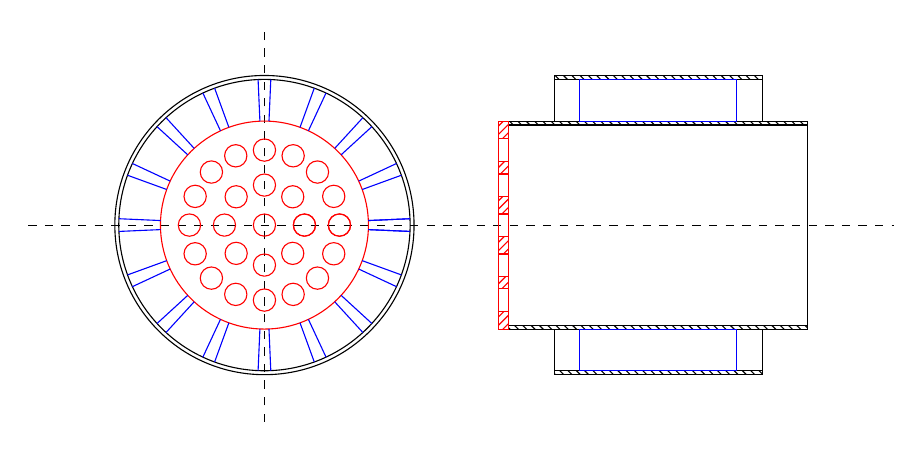
\begin{tikzpicture}

\draw [thin, dashed] ( -3, 0 ) -- ++( 11, 0 );
\draw [thin, dashed] ( 0, -2.5 ) -- ++( 0, 5 );

% Top view
% Perforated plate
\draw [red] ( 0, 0 ) circle ( 2.6416/2 );

\draw [red] ( 0, 0 ) circle ( 0.28194/2 );
\foreach \theta in { 0, 45, ..., 360 }
  \draw [red] ( \theta : 0.508 ) circle ( 0.28194/2 );
\foreach \theta in { 0, 22.5, ..., 360 }
  \draw [red] ( \theta : 0.9525 ) circle ( 0.28321/2 );

% Outer edge
\draw ( 0, 0 ) circle ( 3.8/2 );
\draw ( 0, 0 ) circle ( 1.85 );

% Vanes
\foreach \theta in { 0, 22.5, ..., 360 } {
  \draw [blue] ( \theta - 2.5 : 1.3208 ) -- ( \theta - 2.5 : 1.85 );
  \draw [blue] ( \theta + 2.5 : 1.3208 ) -- ( \theta + 2.5 : 1.85 );
}

% Side View
% Inner edge
\draw ( 5 - 1.9, -1.3208 ) rectangle ++( 3.8, 2.6416 );
\draw [pattern = north west lines] ( 5 - 1.9, -1.3208 ) rectangle ++( 3.8, 0.05 );
\draw [pattern = north west lines] ( 5 - 1.9, 1.3208 ) rectangle ++( 3.8, -0.05 );

% Outer edge
\draw [pattern = north west lines] ( 5 - 1.3208, 1.9 ) rectangle ++( 2.6416, -0.05 );
\draw ( 5 - 1.3208, 1.85 ) rectangle ++( 2.6416, -1.85 + 1.3208 );
\draw [pattern = north west lines] ( 5 - 1.3208, -1.9 ) rectangle ++( 2.6416, 0.05 );
\draw ( 5 - 1.3208, -1.85 ) rectangle ++( 2.6416, 1.85 - 1.3208 );

% Vanes
\draw [blue] ( 4, -1.85 ) rectangle ++( 2, 1.85 - 1.3208 );
\draw [blue] ( 4, 1.85 ) rectangle ++( 2, -1.85 + 1.3208 );

% Perforated plate
\draw [red] ( 5 - 1.9, -1.3208 ) rectangle ++( -0.127, 2.6416 );
\draw [red, pattern = north east lines, pattern color=red] ( 5 - 1.9, -1.3208 ) rectangle ++( -0.127, 0.226695 );
\draw [red, pattern = north east lines, pattern color=red] ( 5 - 1.9, -0.810895 ) rectangle ++( -0.127, 0.161925 );
\draw [red, pattern = north east lines, pattern color=red] ( 5 - 1.9, -0.14097 ) rectangle ++( -0.127, -0.22606 );
\draw [red, pattern = north east lines, pattern color=red] ( 5 - 1.9, 0.14097 ) rectangle ++( -0.127, 0.22606 );
\draw [red, pattern = north east lines, pattern color=red] ( 5 - 1.9, 0.810895 ) rectangle ++( -0.127, -0.161925 );
\draw [red, pattern = north east lines, pattern color=red] ( 5 - 1.9, 1.3208 ) rectangle ++( -0.127, -0.226695 );

\end{tikzpicture}

\caption[Schematic of a vaned swirler]{The figure shows a top and side cross-sectional view of the vaned swirler design used in this study. The perforated plate used to control the relative mass flow split is highlighted in \textcolor{red}{red}, while the vanes used to generate swirl are highlighted in \textcolor{blue}{blue}.}

\label{fig:swirler}

\end{figure}



\subsection{Role of swirl and recirculation zones}

The amount of swirl present in the resulting flow is characterized by a theoretical swirl number, \(S\), which represents the ratio of angular momentum to axial momentum in the flow field.
Cheng et al.\cite{2000-cheng} and later, Littlejohn et al.\cite{2002-littlejohn} reduced this to the following equation.

\begin{equation}
S = \frac{2}{3} \tan \alpha \frac{ 1 - R^3 }{ 1 - R^2 + \left[ M^2\left( \dfrac{1}{R^2} - 1 \right)^2 \right]R^2}
\label{eqn:theoreticalSwirlNumber}
\end{equation}

\nomenclature{\(S\)}{Theoretical swirl number}
\nomenclature[g]{\(\alpha\)}{Swirler vane angle}
\nomenclature{\(R\)}{Diameter ratio of the inner and outer sections of the swirler}
\nomenclature{\(M\)}{Mass flow ratio of the inner and outer regions of the swirler}
  
In Equation \ref{eqn:theoreticalSwirlNumber}, \(R\) is the ratio of the diameter of the central section to the outer diameter of the swirler.
Similarly, \(M\) is the ratio of the mass flow rate through the central portion to the mass flow rate through the outer (vaned) portion of the swirler.
Finally, \(\alpha\) is the angle of the vanes of the swirler.

Along with the recess length of the swirler, the theoretical swirl number was identified to be a key parameter that determines the LSB operating regime.\cite{2002-littlejohn}
Typical values of \(S\) in low swirl combustion range from 0.4--0.6.

Figure \ref{fig:recirculationZones} shows the locations of the notable recirculation zones in the LSB flow field.
The toroidal recirculation zone (TRZ) forms near the inlet, while the central recirculation zone (CRZ) forms within a recirculation bubble along the centerline.
In conventional swirl combustion, the function of the swirl is to induce these recirculation zones that help stabilize the flame by causing a feedback of heat and radicals from the products into the reactants.
In particular, the toroidal recirculation zone traps hot combustion products and continually ignites the reactants at the base of the flame.\cite{2005-johnson}

\begin{figure}

\centering

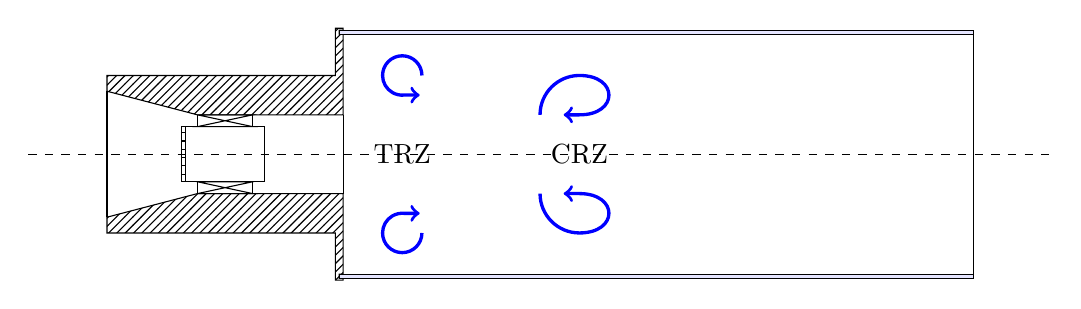
\begin{tikzpicture}

% Nozzle
\draw[pattern=north east lines] ( 0, 0.8 ) -- ++( 1.15, -0.3 ) -- ++( 1.85, 0 ) -- ++( 0, 1.025 ) -- ++( -0.05, 0 ) -- ++( 0, 0.05 ) -- ++( 0.05, 0 ) -- ++( 0, 0.025 ) -- ++ ( -0.1, 0 ) -- ++( 0, -0.6 ) -- ++( -2.9, 0 ) -- cycle;
\draw[pattern=north east lines] ( 0, -0.8 ) -- ++( 1.15, 0.3 ) -- ++( 1.85, 0 ) -- ++( 0, -1.025 ) -- ++( -0.05, 0 ) -- ++( 0, -0.05 ) -- ++( 0.05, 0 ) -- ++( 0, -0.025 ) -- ++ ( -0.1, 0 ) -- ++( 0, 0.6 ) -- ++( -2.9, 0 ) -- cycle;
\draw ( 0, 0.8 ) -- ++( 0, -1.6 );
\draw ( 3, 0.5 ) -- ++( 0, -1 );

% Swirler
\draw ( 1.15, 0.5 ) -- ++( 0.7, 0 ) -- ++( -0.7, -0.15 ) -- ++( 0.7, 0 ) -- ++( -0.7, 0.15 ); 
\draw ( 1.15, 0.5 ) -- ++( 0, -0.15 );
\draw ( 1.85, 0.5 ) -- ++( 0, -0.15 );
\draw ( 1, 0.35 ) rectangle ++( 1, -0.7 );
\draw ( 1.15, -0.5 ) -- ++( 0.7, 0 ) -- ++( -0.7, 0.15 ) -- ++( 0.7, 0 ) -- ++( -0.7, -0.15 ); 
\draw ( 1.15, -0.5 ) -- ++( 0, 0.15 );
\draw ( 1.85, -0.5 ) -- ++( 0, 0.15 );
\draw [pattern = horizontal lines] ( 0.95, 0.35 ) rectangle ++( 0.05, -0.7 );

% Quartz tube
\draw [fill = blue!10!white] ( 2.95, 1.525 ) rectangle ++( 8.05, 0.05 );
\draw [fill = blue!10!white] ( 2.95, -1.525 ) rectangle ++( 8.05, -0.05 );
\draw ( 11, 1.525 ) -- ++( 0, -3.05 );

% Centerline
\draw [dashed, thin] ( -1, 0 ) -- ++( 13, 0 );

% TRZ
\draw [blue, very thick, ->] ( 4, 1 ) arc ( 0 : 275 : 0.25 ) -- ++( 0.2, 0 );
\draw [blue, very thick, ->] ( 4, -1 ) arc ( 0 : -275 : 0.25 ) -- ++( 0.2, 0 );

% CRZ
\draw [blue, very thick, ->] ( 5.5, 0.5 ) arc ( 180 : 90 : 0.5 ) .. controls +( 0.5, 0 ) and +( 0.5, 0 ) .. ++( 0, -0.5 ) -- ++( -0.2, 0 );
\draw [blue, very thick, ->] ( 5.5, -0.5 ) arc ( 180 : 270 : 0.5 ) .. controls +( 0.5, 0 ) and +( 0.5, 0 ) .. ++( 0, 0.5 ) -- ++( -0.2, 0 );

\node at ( 3.75, 0 ) {TRZ};
\node at ( 6, 0 ) {CRZ};

\end{tikzpicture}

\caption[Location of recirculation zones in the LSB flow field]{The figure shows the locations of the recirculation zones in the LSB flow field. The Toroidal Recirculation Zone (TRZ) forms near the abrupt area expansion. The Central Recirculation Zone (CRZ) forms within a recirculation bubble along the centerline of the combustor.}

\label{fig:recirculationZones}

\end{figure}



In the LSB flow field, these recirculation zones are not only much weaker, but also, are not intended to play any part in the stabilization of the flame.
Instead, the LSB flame is a freely propagating turbulent flame that is stabilized by the divergent flow coming from the inlet nozzle.
The function of the swirl in the LSB flow field is merely to enhance this divergence.
This purely aerodynamic means of stabilizing the flame differentiates the LSB regime from conventional swirl combustion.

\subsection{Axial velocity profile and self-similarity}
\label{subsec:lsb-axial-velocity-profile}

The mean axial velocity profile along the centerline of the LSB has been found\cite{2006-cheng,2008-cheng-a} to exhibit a characteristic linear profile in the near field of the inlet.
Two parameters can be used to characterize this linear profile.
First, extrapolating the velocity profile to the point upstream where the axial velocity equals the reference velocity, one can obtain the location of the virtual origin.
The virtual origin represents the point upstream from which the divergence seemingly originates.
The second parameter is the axial stretch rate, which is the slope of the linear region of the axial velocity profile.

Cheng et al.\cite{2006-cheng,2008-cheng-a} investigated these two parameters using a non-preheated setup at atmospheric pressure.
They found that the virtual origin for reacting LSB flow fields asymptotically translates upstream at low/moderate Reynolds numbers, while the mean axial stretch rate, when normalized by the reference velocity, is nearly independent of the same parameter.
This means that at moderately increasing Reynolds numbers, the divergent flow structure shifts upstream into the injector.
This upstream shift ceases for high Reynolds numbers (above 70,000).

Since this shift does not affect the slope of the velocity profile, the researchers plotted the mean axial velocity profiles for different operating conditions, shifted to have a common virtual origin.
Further, the velocity profiles were normalized by the mass-averaged inlet velocity (called the reference velocity).
The resultant plot showed that the linear section of the divergent flow was self-similar at all the velocities tested.
This self-similarity of the mean axial velocity profile was used to explain other observations regarding the flame characteristics, as described in the following sections.

\subsection{Flame stabilization mechanism}
\label{subsec:lsb-flame-stabilization-mechanism}

The flame stabilization mechanism in the LSB is purely aerodynamic.
The turbulent flame is not anchored in the sense of an attached flame, but freely propagates into the reactants.
Conventionally, attached flames are preferred in combustion systems as lifted flames are associated with unstable/undesirable characteristics like blow off.
However, previous studies\cite{2005-johnson} indicate the LSB flame is robustly stabilized and not prone to blow off.

The location where the LSB flame is stabilized is found from the equilibrium condition for flame stabilization---the local reactant velocity, \(U\) equals the local turbulent flame propagation velocity, \(S_T\).
In the LSB, the decrease in the local reactant velocity along the centerline of the combustor is accompanied by an increase in the local turbulence level.
In other words, along the axis of the combustor, at the location where the flame is stabilized, the reactant velocity is decreasing, while the turbulent flame propagation velocity (which scales with the local turbulence) is increasing.

\nomenclature{\(U\)}{Mean local axial velocity of the reactants}
\nomenclature{\(S_T\)}{Turbulent flame speed}

This sets up a stable equilibrium for the flame as shown in Figure \ref{fig:flameEquilibrium}.
Small perturbations causing the flame to move upstream are offset by the increased reactant velocity, while similar perturbations downstream are counteracted by the increased turbulent flame speed.
This is the mechanism behind the robust stabilization of the LSB flame.

\begin{figure}

\centering

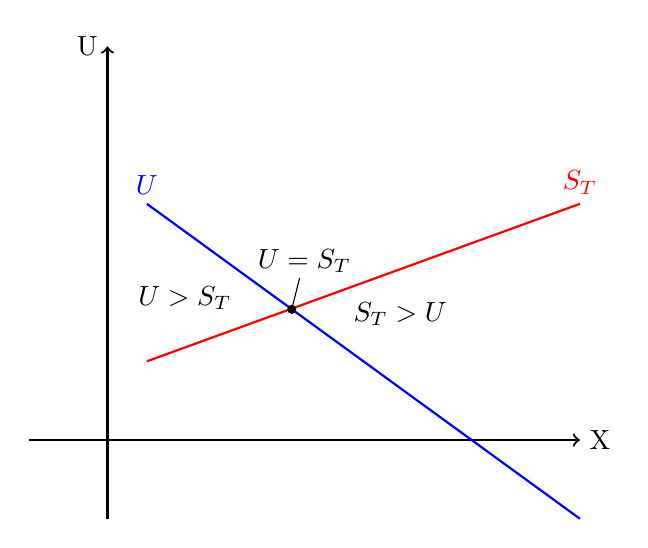
\begin{tikzpicture}

% Axes
\draw [->, thick] ( -1, 0 ) -- ++( 7, 0 );
\draw [->, thick] ( 0, -1 ) -- ++( 0, 6 );

% U profile
\draw [blue, thick] ( 0.5, 3 ) -- ++( 5.5, -4 );

% S_T profile
\draw [red, thick] ( 0.5, 1 ) -- ++( 5.5, 2 );

% Flame stabilization location
\filldraw ( 2.34, 1.66 ) circle ( 0.05 ) -- ++( 0.1, 0.4 );

% Labels
\node at ( 6, 0 ) [right] {X};
\node at ( 0, 5 ) [left] {U};

\node at ( 0.5, 3 ) [above,blue] {\(U\)};
\node at ( 6, 3 ) [above, red] {\(S_T\)};

\node at ( 2.5, 2 ) [above] {\(U=S_T\)};
\node at ( 1.7, 1.8 ) [left] {\(U>S_T\)};
\node at ( 3, 1.6 ) [right] {\(S_T>U\)};

\end{tikzpicture}

\caption[Schematic of LSB flame stabilization]{The figure above illustrates the robustness of the LSB flame stabilization mechanism. The flame is stabilized at the point where the reactant velocity, \(U\), and the turbulent flame speed, \(S_T\), are equal. Perturbations to the flame standoff distance to the left or the right are counteracted by either \(U\) or \(S_T\) respectively making this a stable equilibrium.}

\label{fig:flameEquilibrium}

\end{figure}



\subsection{Effect of Flow Parameters on Flame Characteristics}

The operating conditions of the LSB combustor are fully described by four fundamental flow parameters; the combustor pressure, \(p\), the combustor temperature, \(T\), the mixture equivalence ratio, \(\phi\), and the reference velocity, \(U_0\).
The reference velocity represents the mass-averaged velocity of the reactants entering the LSB and is defined after Cheng et al.\cite{2000-cheng} as a function of several variables such as the mass flow rates of the air and fuel, \(\dot{m}\), their densities at the swirler, \(\rho\) and the area of the swirler calculated from its outer diameter, \(d_s\).

\begin{equation}
U_0 = \frac{ \left( \dfrac{ \dot{m}_{air} }{ \rho_{air} } \right) + \left( \dfrac{ \dot{m}_{fuel} }{ \rho_{fuel} }\right) }{ \dfrac{\pi d_s^2 }{4} }
\label{eqn:referenceVelocity}
\end{equation}

\nomenclature{\(p\)}{Combustor pressure}
\nomenclature{\(T\)}{Preheat temperature}
\nomenclature[g]{\(\phi\)}{Equivalence ratio}
\nomenclature{\(U_0\)}{Reference velocity}
\nomenclature{\(\dot{m}\)}{Mass flow rate}
\nomenclature[g]{\(\rho\)}{Density}
\nomenclature{\(d_s\)}{Outer diameter of the swirler}

In this section, we will briefly discuss the effect of flow parameters have on the flame characteristics of interest.
By way of an example, and as a means to introduce a few basic concepts, the following discussion will examine the effect of increasing the reference velocity on the flame location, shape and structure.
In-depth discussion of the dependence of each flame characteristic on all the flow parameters of interest will be deferred until Chapter \ref{ch:lsb}.

\subsubsection{Effect on Flame Standoff Distance}
\label{subsubsec:flame-characteristics-standoff}

As described earlier in Section \ref{subsec:lsb-flame-stabilization-mechanism}, the LSB flame is stabilized where the local reactant velocity and turbulent flame speed are equal.
Unlike the laminar flame speed, \(S_L\), the turbulent flame speed is not uniquely determined by the reactant composition and thermodynamic conditions.
Instead, it is a function of the flow characteristics and the burner geometry.

\nomenclature{\(S_L\)}{Laminar flame speed}

A simple model proposed by Damk{\"o}hler\cite{1940-damkohler} treats the turbulent flame as a wrinkled laminar flame.
The presence of these wrinkles vastly increases the surface area of the flame, increasing the rate at which the reactants can be consumed through the flame.
The size of these wrinkles can be related to the rms of the local reactant velocity, \(u\).
Expressed mathematically, this leads to Equation \ref{eqn:damkohlerModel}.

\begin{equation}
\frac{ S_T }{ S_L } = 1 + \frac{ u }{ S_L }
\label{eqn:damkohlerModel}
\end{equation}

\nomenclature{\(u\)}{rms of the local axial velocity of the reactants}

Cheng et al.\cite{2002-cheng,2009-cheng,2010-littlejohn} observed that the slope of this linear relationship was dependent on the fuel mixture being used.
This idea is encapsulated in Equation \ref{eqn:chengModel} that presents a modified version of Equation \ref{eqn:damkohlerModel}.

\begin{equation}
\frac{ S_T }{ S_L } = 1 + K \frac{ u }{ S_L }
\label{eqn:chengModel}
\end{equation}

\nomenclature{\(K\)}{Linearity constant in the turbulent flame speed model}

The constant \(K\) has a value of around 1.73 for methane-air mixtures and a somewhat higher value---3.15---for hydrogen-air mixtures,\cite{2009-cheng} suggesting that the turbulent flame speed is affected strongly by the thermo-diffusive properties of the fuel.

In order to predict the expected effect of increasing the reference velocity, consider the following analysis at the flame standoff location where \(U\)=\(S_T\).

\begin{align}
\frac{ S_T }{ S_L } &= 1 + K \frac{ u }{ S_L } \nonumber \\
S_T &= S_L + K u \nonumber \\
\implies U &= S_L + K u \nonumber \\
U_0 - \frac{ dU }{ dx } ( X_f - X_0 ) &= S_L + K u \nonumber \\
  \therefore X_f &= X_0 + \frac{1 - \left( \dfrac{ S_L }{ U_0 } + K\dfrac{ u }{ U_0 } \right) }{ \dfrac{ 1 }{ U_0 } \dfrac{ dU }{ dx } }
\label{eqn:flameImmobility}
\end{align}

\nomenclature{\(X_f\)}{Location of the flame standoff point measured from the inlet}
\nomenclature{\(X_0\)}{Location of the virtual origin measured from the inlet}

Consider the terms on the RHS of Equation \ref{eqn:flameImmobility}.
As described in Section \ref{subsec:lsb-axial-velocity-profile}, the virtual origin location is invariant for moderate to high values of reference velocity.
In the same section, the normalized slope of the velocity profile, \(\dfrac{ 1 }{ U_0 } \dfrac{ dU }{ dx }\), was also noted as being invariant with reference velocity.
In the numerator of the second term, the local turbulence intensity, \(\dfrac{ u }{ U_0 }\), can also be expected to be a constant, since \(u\) should scale with the reference velocity in the same manner as long as the burner geometry does not change.
The turbulence intensity, \(\dfrac{ u }{ U_0 }\) in the LSB increases from the inlet along the centerline reaching values on the order of 0.1--1.0 near the flame standoff location.\cite{2008-cheng-a}
That leaves only the term \(\dfrac{ S_L }{ U_0 }\) as a function of \(U_0\).
Typically, the laminar flame speeds are at least an order of magnitude, if not more, lower (\(\approx O(1)\) m/s) than the reference velocities at which the LSBs are operated (\(\approx O(10)\) m/s).
As a result, variations in this term are a vanishingly small portion of the sum, leaving the entire RHS independent of \(U_0\).
%SAME COMMENT AS LAST TIME - BOTH TERMS IN THE ( ) MAY BE OF THE SAME ORDER (0.1), THEN HOW CAN YOU NEGLECT THE FIRST TERM? ARE YOU REALLY SAYING Xf~Xo+ Uo/(dU/dx)?
In other words, the flame location, \(X_f\) is expected to be invariant with the reference velocity at which the LSB is operated.

\subsubsection{Effect on Flame Shape}

Now, consider the effect of increasing the reference velocity on the angle of the flame cone.
Again, the stabilization condition is equality between the local velocity and the turbulent flame speed.
However, along the flame cone, the reactant velocities are much higher and the flame propagation can only occur at an angle to the reactant velocity.
Increasing the reference velocity does not affect any of these factors and thus, the flame angle can also be expected to be unchanged at higher reference velocities.

\subsubsection{Effect on Flame Structure}

Finally, the effect of the reference velocity on the structure of the turbulent flame should be considered.
Depending on the characteristics of the flame structure, the operation point can be placed on a Borghi diagram, as shown in Figure \ref{fig:borghiDiagram}.
The Borghi diagram\cite{1985-borghi} is a phase diagram used to classify and delineate regimes of premixed turbulent combustion.
The double-log plot is drawn using properties of the reacting mixture and its turbulence-related quantities.
It is partitioned into various regimes by different straight lines representing the locus of non-dimensional parameters.
It is useful to examine the effect of various parameters on the flame structure by examining the tendency of the operating point to shift on the Borghi diagram.

\begin{figure}

\centering

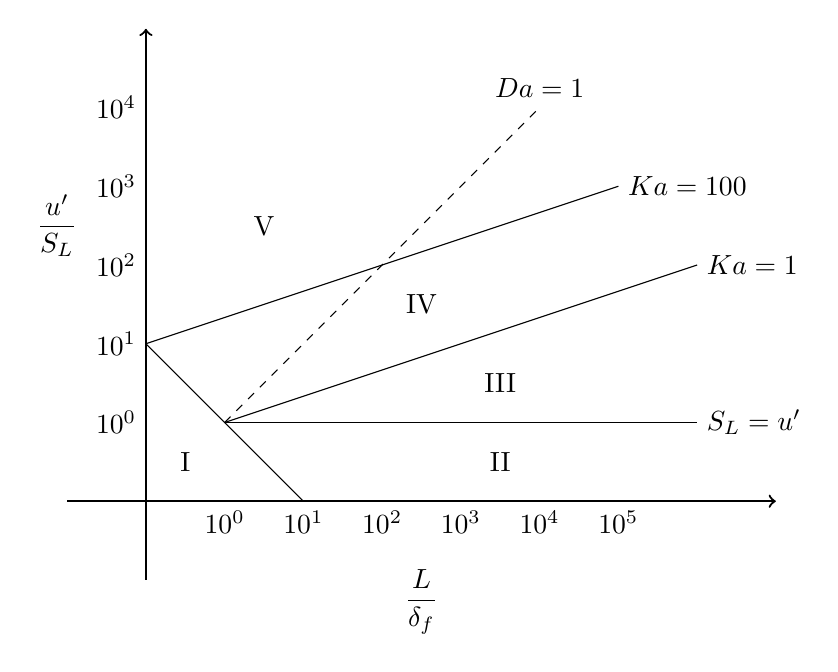
\begin{tikzpicture}

% Axes
\draw [->, thick] ( -1, 0 ) -- ++( 9, 0 );
\draw [->, thick] ( 0, -1 ) -- ++( 0, 7 );

% Regimes
\draw ( 0, 2 ) -- ++( 2, -2 );
\draw ( 1, 1 ) -- ++( 6, 0 );
\draw [dashed] ( 1, 1 ) -- ++( 4, 4 );
\draw ( 1, 1 ) -- ++( 6, 2 );
\draw ( 0, 2 ) -- ++( 6, 2 );

% Labels
\node at ( 0.5, 0.5 ) {I};
\node at ( 4.5, 0.5 ) {II};
\node at ( 4.5, 1.5 ) {III};
\node at ( 3.5, 2.5 ) {IV};
\node at ( 1.5, 3.5 ) {V};

\foreach \x in { 0, ..., 5 }
  \node at ( \x + 1, 0 ) [below] {\(10^\x\)};
\foreach \y in { 0, ..., 4 }
  \node at ( 0, \y + 1 ) [left] {\(10^\y\)};

\node at ( 3.5, -0.75 ) [below] {\(\dfrac{ L }{ \delta_f }\)};
\node at ( -0.75, 3.5 ) [left] {\(\dfrac{ u' }{ S_L }\)};

\node at ( 7, 1 ) [right] {\(S_L = u'\)};
\node at ( 7, 3 ) [right] {\(Ka = 1\)};
\node at ( 6, 4 ) [right] {\(Ka = 100\)};
\node at ( 5, 5 ) [above] {\(Da = 1\)};

\end{tikzpicture}

\caption[Borghi diagram]{The figure shows the Borghi diagram marking the various regimes of premixed turbulent combustion---I. laminar flames, II. wrinkled flamelets, III. corrugated flamelets, IV. thin flame zones, and V. broken reaction zones---separated by contours of Karlovitz number.}

\label{fig:borghiDiagram}

\end{figure}



Several versions of the Borghi diagram exist that use different variables to plot the combustion regimes.
In the current study, we use a diagram based on \(\dfrac{ u }{ S_L }\) and \(\dfrac{ L }{ \delta_f }\).
The key parameters to be considered here are the rms velocity, \(u\), the laminar flame speed, \(S_L\), the integral length scale of the flow, \(L\), and the flame thickness, \(\delta_f\).

\nomenclature{\(L\)}{Integral length scale}
\nomenclature[g]{\(\delta_f\)}{Thickness of the flame}

Increasing the reference velocity will be accompanied with a concomitant increase in the level of turbulence in the flow, but it changes none of the other parameters.
As a result, the operating point will traverse vertically on the Borghi diagram.
If the LSB operates in the wrinkled flamelets regime to begin with, at very high reference velocities, it may be expected to cross over into the corrugated flamelets regime.
This will be marked by the formation of holes and pockets in the flame sheet.
%SO THE READER WILL BE EXPECTING YOU TO POINT THIS OUT IN CHAPTER 5!

\section{CH PLIF Signal Modeling}
\label{sec:background-chplif-signal-modeling}

While the intent and scope of this work is to use CH PLIF as a visualization technique to image the flame front with high fidelity, it would be extremely useful to be able to predict the CH PLIF signal intensity for different reactant mixtures and initial conditions as a means to gauge the feasibility of applying the technique to acquire high fidelity images of the flame at those conditions.
To that end, this discussion will attempt to develop a mathematical model to calculate, in a semi-quantitative manner, the rate of CH PLIF photons emitted by the illuminated reaction zone.
The following discussion introduces important concepts in LIF signal intensity calculation using a simple two-level model and then proceeds to apply these concepts to model the more complicated physical processes in the CH system.

\subsection{Basic Model}
\label{subsec:chplif-basic-model}

In its most basic form, the rate at which fluorescence photons are generated in a system, \(\Phi\) is the product of the number of emitters, \(N\) and the Einstein coefficient for spontaneous emission, \(A\).

\begin{equation}
  \Phi = N\times A
  \label{eqn:fluorescencePhotons}
\end{equation}

\nomenclature[g]{\(\Phi\)}{Photon counts per second}
\nomenclature{\(N\)}{Number of fluorescence emitters}
\nomenclature{\(A_{ij}\)}{Einstein coefficient for spontaneous emission between levels \(i\) and \(j\)}

The fluorescence photons produced are radiated in all directions and only a fraction of these can be recorded by a collection system in an experiment.
This fraction is determined by the experimental set up, the collection angle, and the efficiency of the optics and the detector used to record the signal.
For this analysis, however, this fraction is omitted to reduce complexity.

In a simple two-level model for the fluorescing system, as shown in Figure \ref{fig:twoLevel}, Equation \ref{eqn:fluorescencePhotons} may be expanded in terms of the number density of the emitters, \(n\), and the volume in which the fluorescence occurs, \(V\).

\begin{equation}
  \Phi = n_1VA_{10}
\end{equation}

\nomenclature{\(n\)}{Number density of molecules}
\nomenclature{\(V\)}{Volume}

\begin{figure}

\centering

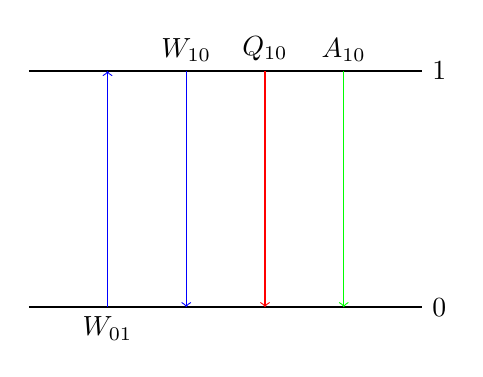
\begin{tikzpicture}

% Lower state
\draw [thick] ( 0, 0 ) -- ++( 5, 0 );

% Upper state
\draw [thick] ( 0, 3 ) -- ++( 5, 0 );

% Transitions
\draw [blue, ->] ( 1, 0 ) -- ++( 0, 3 );
\draw [blue, ->] ( 2, 3 ) -- ++( 0, -3 );
\draw [red, ->] ( 3, 3 ) -- ++( 0, -3 );
\draw [green, ->] ( 4, 3 ) -- ++( 0, -3 );

\node at ( 5, 0 ) [right] {0};
\node at ( 5, 3 ) [right] {1};

\node at ( 1, 0 ) [below] {\(W_{01}\)};
\node at ( 2, 3 ) [above] {\(W_{10}\)};
\node at ( 3, 3 ) [above] {\(Q_{10}\)};
\node at ( 4, 3 ) [above] {\(A_{10}\)};

\end{tikzpicture}

\caption[Transitions in a basic two-level model for fluorescence]{The figure shows energy levels and transitions between two levels, labeled 0 and 1, in a basic model of laser-induced fluorescence. Stimulated absorption and emission are shown in \textcolor{blue}{blue}, collisional quenching is shown in \textcolor{red}{red} and spontaneous emission is shown in \textcolor{green}{green}.}

\label{fig:twoLevel}

\end{figure}



The population of the upper state, \(n_1\) can be solved for by rate analysis.
The mathematical treatment is not particularly complicated and is covered in detail by various textbooks and review papers.\cite{1996-eckbreth,1997-daily}
Here, we shall merely remark that the functional form of the solution has two limiting cases.
The limits are decided by the relative magnitudes of the pumping rate, \(W_{01}\), which depends on the laser intensity and the radiative transition probability, and the relaxation rate in the absence of an external field, which is given by the sum of the spontaneous emission and collisional quenching rate, \(A_{10} + Q_{10}\).
The pumping rate is the rate at which the upper energy level is populated through stimulated absorption from the lower level.
The relaxation of the molecules to the lower energy state occurs either through spontaneous emission of a photon or energy transfer to other molecules through inelastic collisions.

When the pumping rate is far lower compared to the relaxation processes (\(W_{01} \ll A_{10} + Q_{10}\)), the solution tends to the weak excitation limit.
In this limit, the functional form of the solution is shown in Equation \ref{eqn:twoLevelModel-weak}

\begin{equation}
  \Phi = n_0 V W_{01}\overbrace{\frac{A_{10}}{A_{10}+Q_{10}}}^{\text{Fluorescence Yield}}
  \label{eqn:twoLevelModel-weak}
\end{equation}

\nomenclature{\(W_{ij}\)}{Rate of pumping of molecules from level \(i\) to level \(j\)}
\nomenclature{\(Q_{ij}\)}{Rate of collisional quenching of excited molecules from level \(i\) to level \(j\)}

The \(n_0VW_{01}\) term in Equation \ref{eqn:twoLevelModel-weak} represents the number of molecules that are excited to the upper state per second, while the fluorescence yield represents the fraction of these molecules that will produce a LIF signal.
In typical combustion environments, the fluorescence yield is usually small, since the collisional quenching rate dominates the spontaneous emission rate.
The rate of collisional quenching of the fluorescing species by another species in the flame is proportional to the frequency of collisions between the two.
Further, the effectiveness of such collisions is decided by a collision cross-section, \(\sigma\), which is often a function of the temperature.
Equation \ref{eqn:quenchingRate} presents the calculation of the collisional quenching rate by summation over all the species, \(i\), in the flame.

\begin{align}
  Q_{10} &= \sum_i n_i \times \sigma_i \times \bar{c_i} \nonumber \\
  & = \sum_i n_i \sigma_i \sqrt{\frac{8kT}{\pi\mu_i}} \nonumber \\
  & = \sqrt{\frac{8kT}{\pi}} \sum_i \frac{n_i \sigma_i}{\sqrt{\mu_i}}
  \label{eqn:quenchingRate}
\end{align}

\nomenclature[g]{\(\sigma_i\)}{Collisional quenching cross-section of species \(i\)}
\nomenclature{\(\bar{c}\)}{Average velocity} 
\nomenclature{\(k\)}{Boltzmann constant}
\nomenclature[g]{\(\mu_i\)}{Reduced mass of species \(i\)}

In Equation \ref{eqn:quenchingRate}, \(k\) is the Boltzmann constant, \(T\) is the local temperature, \(n_i\) is the number density of species \(i\) and \(\mu_i\) represents the reduced mass of the colliding molecules, given by Equation \ref{eqn:reducedMass}.

\begin{equation}
  \mu_i = \frac{ m_i m }{ m_i + m }
  \label{eqn:reducedMass}
\end{equation}

\nomenclature{\(m\)}{Mass}

In Equation \ref{eqn:reducedMass}, \(m\) is the mass of the marker species, while \(m_i\) are the masses of the colliding species.
Since LIF in combustion primarily targets minor species, by probability, these collisions will almost always occur with major species in the system.
As a result, the summation in Equation \ref{eqn:quenchingRate} need only be carried out over the major species in the flame.
The values of the local number densities of the major species can be measured by techniques like Raman scattering, or can be obtained from solving chemical kinetics models.

\subsubsection{Absorption Integral Calculation}
\label{subsubsec:basic-model-absorption-integral-calculation}

Let us now briefly examine the first term in Equation \ref{eqn:twoLevelModel-weak} in further detail.
Let \(\phi(\nu)\) represent the normalized line shape of the absorption line being excited, such that \(\int \phi(\nu) d\nu = 1\).
If \(B_{01}\) is the Einstein coefficient for absorption for the line being excited, the term \(B_{01}\phi(\nu)\) represents the spectral absorptivity of the line at \(\nu\).
\(B_{01}\) is usually presented in m\(^2\)/Js for LIF applications.
Similarly, let \(I_\nu\) be the spectral intensity of the incident radiation, which is the intensity (power per area) of the laser beam per spectral interval.
Let \(\psi(\nu)\) be the normalized spectral profile of the laser lineshape, such that \(I_\nu\) = \(I \psi(\nu)\) and \(\int \psi(\nu) d\nu = 1\).
\(I_\nu\) is usually given in W/cm\(^2\)/cm\(^{-1}\) for ease of use in laser applications.

\nomenclature[g]{\(\nu\)}{Wavenumber}
\nomenclature[g]{\(\phi(\nu)\)}{Normalized line shape of an absorption line}
\nomenclature[g]{\(\psi(\nu)\)}{Normalized line shape of the laser beam}
\nomenclature{\(B_{ij}\)}{Einstein coefficient for stimulated absorption from level \(i\) to level \(j\)}
\nomenclature{\(I_\nu\)}{Spectral intensity of the laser beam}

The product of the spectral absorptivity and the spectral intensity integrated over the spectrum, gives the pumping rate, \(W_{01}\), as shown in Equation \ref{eqn:pumpingRate-unsimplified}.
The factor \(c\) is the speed of light, which brings the units of \(W_{01}\) to s\(^{-1}\).

\begin{equation}
  W_{01} = \frac{I}{c} \int \psi(\nu) B_{01}\phi(\nu) d\nu
  \label{eqn:pumpingRate-unsimplified}
\end{equation}

\nomenclature{\(c\)}{Speed of light in vacuum}

\subsubsection{Population Distribution}
\label{subsubsec:basic-model-population-distribution}

Once again, consider Equation \ref{eqn:twoLevelModel-weak}, this time focusing on the term \(n_0\), the number density of the marker species in the lower energy state that are available for excitation to the upper state.
In reality, this comprises only a small subset of all the available molecules of the marker species in the system.

\begin{equation}
  n_0 = nf_0
  \label{eqn:boltzmannFraction}
\end{equation}

\nomenclature{\(f_i\)}{Boltzmann fraction of the population at energy level \(i\)}

In Equation \ref{eqn:boltzmannFraction}, \(n\) is the number density of all marker species over all the energy levels, while the fraction, \(f_0\), represents the proportion of the marker species that populates the lower energy level.

\subsubsection{Solution}
\label{subsubsec:basic-model-solution}

Substituting Equations \ref{eqn:pumpingRate-unsimplified} and \ref{eqn:boltzmannFraction} into \ref{eqn:twoLevelModel-weak}, and noting that the signal produced is actually integrated over a volume,

\begin{equation}
  \Phi = \int_V \frac{n A_{10}}{A_{10} + Q_{10}} \frac{I}{c} f_0 B_{01} \textcolor{red}{\int_\nu \psi(\nu) \phi_j(\nu) d\nu} dV
  \label{eqn:twoLevelModel-unsimplified}
\end{equation}

\nomenclature{\(I\)}{Intensity of the laser beam}

In Equation \ref{eqn:twoLevelModel-unsimplified}, the absorption integral from Equation \ref{eqn:pumpingRate-unsimplified} is highlighted in \textcolor{red}{red}.
The outer integral is performed in space, over the portion of the flame illuminated by the laser sheet.
Under the assumption that the laser intensity is uniformly distributed over the sheet thickness, it is possible to rewrite the outer integral as a 1-D integral over the thickness of the flame by replacing the laser intensity, \(I\) with the laser power, \(P\).

\begin{equation}
  \Phi = \frac{P}{c} \int_x \frac{n A_{10}}{A_{10}+Q_{10}} f_0 B_{01} \int_\nu \psi(\nu) \phi_j(\nu) d\nu dx
  \label{eqn:twoLevelModel}
\end{equation}

\nomenclature{\(P\)}{Power of the laser beam}

Equation \ref{eqn:twoLevelModel} is thus, the solution to the two-level model in the weak excitation limit.
Note that the LIF signal varies linearly as the incident laser power (or intensity).
Consequently, the weak excitation limit is also referred to as the linear regime.

For the sake of completion, we will briefly mention the other limit of the two-level model solution that occurs when the rate of pumping far exceeds the relaxation rate (\(W_{01} \gg A_{10} + Q_{10}\)).
This is called the saturated limit and in this limit, the fluorescence signal ceases to change with the intensity of the incident laser beam.
Operating in this regime has one major advantage for quantitative LIF measurements; the measured fluorescence signal is nearly independent of the collisional quenching rate, a parameter that can change significantly throughout the combustion.
However, there are several drawbacks to operating in this regime.
First, the magnitude of the LIF signal per unit incident laser intensity tends to be the maximum in the linear regime.
Once the variation ceases to be linear (even before nearing the saturation limit), we get diminishing returns for increasing the laser power.
For measurements with low signal-to-noise ratio, which is often the case for PLIF imaging, this is a significant drawback.
Further, the saturation criterion (maintaining a high laser intensity) is difficult to satisfy simultaneously in the spatial, temporal and spectral domains.
For these reasons, we will restrict our discussion hence forward the linear regime only.

\subsection{CH PLIF Process}
\label{subsec:background-ch-plif-process}

In this section, we will examine the limitations of trying to apply the two-level model to describe the CH PLIF process.

Laser-Induced Fluorescence is a multi-step process.
First, the marker species absorbs a photon and transitions from a lower energy state to a higher one.
This is followed by several physical processes, of which only one pathway leads to the spontaneous de-excitation of the excited molecule, accompanied by the release of a photon.
The de-excitation can---but does not need to---take the molecule back to the original state.
If the molecule does return to its original state, the fluorescence is said to be resonant.
Due to the difficulty of measuring fluorescence signals at the same wavelength as the excitation beam, most practical applications of LIF tend to be non-resonant.
The choice of the spectral and temporal properties of the excitation laser source, and of the detected fluorescence emission, constitute the excitation and detection schemes.

The excitation scheme chosen for this study follows the work done by Li et al.\cite{2007-li-a} who used a ring-cavity, pulsed alexandrite laser to provide excitation in the vicinity of the R-bandhead of the CH \(B^2\Sigma^- \leftarrow X^2\Pi\) (0,0) system.
This bandhead, shown in Figure \ref{fig:chB-XAbsorption}, is found at a frequency of about 25824 cm\(^{-1}\ (or a wavelength of about 387.2 nm) and represents transitions from a ground state rotational quantum number of \(N''=7\).
When operated in multimode, alexandrite lasers have relatively large bandwidths (a few cm\(^{-1}\) is not uncommon) and hence make it possible to excite several of the neighboring transitions near the bandhead.

\nomenclature{\(N''\)}{Total rotational quantum number (of the lower level)}

\begin{figure}

\centering

\input{figures/chB-XAbsorptionPlot}

\caption[CH \(B^2\Sigma^-\leftarrow X^2\Pi\) (0,0) R-bandhead absorption lines]{The figure shows the frequencies of the absorption lines near the R-bandhead of the CH \(B^2\Sigma^-\leftarrow X^2\Pi\) (0,0) band. The individual lines are labeled with corresponding \(N''\) quantum number.}

\label{fig:chB-XAbsorption}

\end{figure}



Upon excitation, these molecules transition to the second electronically excited \(B^2\Sigma^-\) state and populate the lowest vibrational level, (\(v'=0\)).
At this point, the following possibilities exist for the excited molecule:

\nomenclature{\(v\)}{Vibrational quantum number}

\begin{enumerate}
  \item The molecule can undergo inelastic collisions with other molecules, resulting in relaxation in the rotational, vibrational or electronic manifolds.
  \item The molecule can spontaneously emit a photon and return to any of the lower energy states.
  \item The molecule can experience stimulated emission in the presence of another photon of the appropriate frequency and return to any of the lower energy states.
  \item The molecule can experience further excitation either by absorbing a photon or through collisional means and can react chemically.
\end{enumerate}

Now, let us examine these potential pathways in greater detail.
The first pathway pertains to relaxation.
The excitation and subsequent population of a higher energy state causes the CH population distribution to deviate from the equilibrium Boltzmann distribution.
The degree of relaxation possible is limited by the lifetime of the energy level the excited species occupy. 
The maximum time possible for relaxation is given by the collision-free, radiative lifetime of the \(B\) electronic state, which is about 300 ns\cite{1996-luque-c}---long enough for sufficient rotational relaxation to occur, but too short for complete vibrational relaxation.
Based on experiments conducted by Garland et al.\cite{1985-garland-b}, it is estimated that the vibrational energy transfer between the two bound states available to the \(B^2\Sigma^-\) state is about two orders of magnitude slower than the rotational energy transfer.
As a result, we may suppose that the vibrational manifold remains relatively unaffected, while the rotational manifold can partially relax toward an equilibrium distribution.
The question of the electronic relaxation will be addressed later in this discussion.

The second option available for the excited CH molecule is to spontaneously emit a photon and return to a lower energy state.
Spontaneous de-excitation to the ground state primarily follows the diagonal \(B^2\Sigma^-\rightarrow X^2\Pi\) (0,0) band.
The rate of such spontaneous emission between two states is given by the Einstein emission coefficient for the transition.
Once again, we will defer discussion of the \(B-A\) transition until later in this discussion.

The third option is for the CH molecule to experience stimulated emission in the presence of a photon of an appropriate frequency.
It is highly unlikely that the apposite photon would have a frequency other than the excitation laser.
The rate of stimulated emission induced by the excitation laser beam is proportional to the Einstein absorption coefficient for the transition.
Other photons that can induce stimulated emission could originate from spontaneous emission or CH* chemiluminescence, however they would be negligible in intensity compared to the laser.

The fourth option is for the molecule to experience further excitation by absorbing multiple photons or through collisions with other energetic molecules in the system.
Since most available photons do not match any transitions from the \(B^2\Sigma^-\), \(v=0\) state, it is unlikely to experience multi-photon excitation.
However, collisional removal of CH molecules from the \(B\) state is certainly possible.

Having listed all the options, let us resume the discussion on the possibility of electronic energy transfer from the excited \(B^2\Sigma^-\), \(v'=0\) state.
The spacing of the energy levels in the CH system, shown in Figure \ref{fig:chRKR}, is such that the \(B^2\Sigma^-\), \(v'=0\) state is found to be near-degenerate with the \(A^2\Delta\), \(v=1\) energy level.
Consequently, the \(B^2\Sigma^-\leftrightarrow A^2\Delta\) (0,1) transition is reversible.
Due to this, collisional population of the \(A^2\Delta\) \(v=0,1\) states from the \(B^2\Sigma^-\) \(v=0\) state occurs rapidly.
Garland et al.\cite{1985-garland-b} measured that these transfers account for almost a quarter of all collisional depletion of the \(B^2\Sigma^-\), \(v=0\) level.
Theoretical calculations using overlap integrals between the involved energy levels predict that a majority of these transfers will be along the diagonal (0,0) transition.\cite{2000-luque}.
Instead, experimental data indicates that the number is closer to a fifth, with almost 80\% of the transfers following the near-degenerate (0,1) pathway.

\begin{figure}

\centering

\input{figures/chRKRPlot}

\caption[Potential curves for the CH system]{The figure shows the RKR potential curves for the \(X^2\Pi\), \(A^2\Delta\) and \(B^2\Sigma^-\) energy levels in the CH system. A few vibrational levels are indicated for the \(X^2\Pi\) and \(A^2\Delta\) states. The \(B^2\Sigma^-\) state has only two bound vibrational levels. The diagram is reproduced from Richmond et al.\cite{2005-richmond} who based it on \emph{ab initio} calculations by van Dishoeck\cite{1987-vandishoeck}}

\label{fig:chRKR}

\end{figure}



It is this electronic energy transfer mechanism that enables our excitation scheme to record high quality CH PLIF images.
Having now populated the \(A^2\Delta\) states, the resulting spontaneous emission from the \(A^2\Delta\rightarrow X^2\Pi\) (0,0) and (1,1) transitions can be easily observed between 420--440 nm.
A small portion of the fluorescence in this wavelength range also occurs from the \(B^2\Sigma^-\rightarrow X^2\Pi\), (0,1) transition.
Since these emission wavelengths are located far from the excitation wavelength, a simple glass filter is sufficient to suppress any elastic scattering from the laser beam.

\subsection{Improved Model}
\label{subsec:chplif-improved-model}

While the two-level model is conceptually simple, applying it to describe the complicated physical process of CH PLIF is challenging.
Daily\cite{1997-daily} notes, for example, that significant errors can result from using the two-level model to describe even a three-level system.
Hence, it is worthwhile to investigate a more complicated model that can describe the CH system with higher fidelity.

Figure \ref{fig:energyLevels} shows the relevant pathways that lead to the fluorescence emission as discussed in Section \ref{subsec:background-ch-plif-process}.
An accurate model of the CH system should involve at least five energy levels, namely the \(B^2\Sigma^-\), \(v=0\), \(A^2\Delta\), \(v=0,1\), and \(X^2\Pi\), \(v=0,1\) levels.
The model will need to account for collisional transfers between each of these levels, in addition to spontaneous and stimulated transitions.
By limiting the model to five levels, we are assuming that the distributions within the rotational manifolds associated with each vibrational level do not play a significant role in altering the net rate of transfer between vibration levels.
Even for just five levels, the mathematical solution quickly becomes tedious and complicated.
Further, it involves several rate coefficients that have not yet been measured experimentally.

\begin{figure}

\centering

\begin{tikzpicture}

% Ground states
\draw [thick] ( 3, 0 ) -- ++( 4, 0 );
\node at ( 7, 0 ) [right] {\(X^2\Pi, v = 0\)};
\draw [thick] ( 3, 1 ) -- ++( 4, 0 );
\node at ( 7, 1 )  [right] {\(X^2\Pi, v = 1\)};

% First electronic states
\draw [thick] ( 0, 4 ) -- ++( 3, 0 );
\node at ( 0, 4 )  [left] {\(A^2\Delta, v = 0\)};
\draw [thick] ( 0, 5 ) -- ++( 3, 0 );
\node at ( 0, 5 )  [left] {\(A^2\Delta, v = 1\)};

% Second electronic state
\draw [thick] ( 7, 5 ) -- ++( 3, 0 );
\node at ( 10, 5 )  [right] {\(B^2\Sigma^-, v = 0\)};

% Transitions
\draw [blue, ->] ( 6, 0 ) -- ++( 3, 5 );

\draw [red, ->] ( 6.5, 5 ) -- ++( -3, 0 );
\draw [red, ->] ( 6.5, 4.75 ) -- ++( -3, -0.75 );

\draw [green, ->] ( 8, 5 ) -- ++( -2.25, -4 );
\draw [green, ->] ( 1, 4 ) -- ++( 3, -4 );
\draw [green, ->] ( 1, 5 ) -- ++( 3, -4 );

\end{tikzpicture}

\caption[Relevant transitions in a CH molecule]{Some of the important transitions between energy levels in a CH molecule are shown. The excitation of the CH molecules (\textcolor{blue}{blue}) is followed by collisional energy transfer processes (\textcolor{red}{red}) which populate additional energy levels. Spontaneous emission from some of these energy levels (\textcolor{green}{green}) is collected.}

\label{fig:energyLevels}

\end{figure}



Fortunately, this can be significantly simplified.
Previous studies\cite{1996-luque-c,2000-luque} have indicated that the off-diagonal \(B\rightarrow X\) (0,1) transition plays a relatively minor role accounting for only 3.5\% of the total fluorescence.
Further, the radiative \(A\rightarrow X\) transitions are known\cite{1996-luque-b} to be strongly diagonal, with little or no interaction\cite{1985-garland-b} between the two states.
The net result of these two assertions is that we can treat the two \(B\rightarrow A\rightarrow X\) pathways to be disjoint and parallel.
The resulting model involving four energy levels is shown in Figure \ref{fig:simplifiedEnergyLevels}.

\begin{figure}

\centering

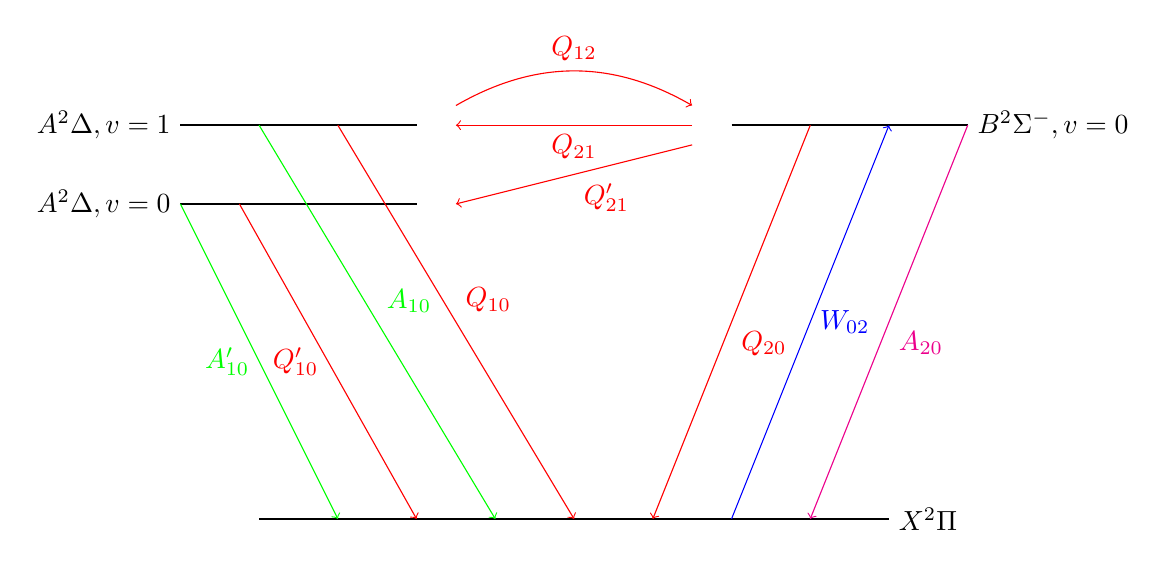
\begin{tikzpicture}

% Ground state
\draw [thick] ( 1, 0 ) -- ++( 8, 0 );
\node at ( 9, 0 ) [right] {\(X^2\Pi\)};

% First electronic states
\draw [thick] ( 0, 4 ) -- ++( 3, 0 );
\node at ( 0, 4 ) [left] {\(A^2\Delta, v = 0\)};
\draw [thick] ( 0, 5 ) -- ++( 3, 0 );
\node at ( 0, 5 ) [left] {\(A^2\Delta, v = 1\)};

% Second electronic state
\draw [thick] ( 7, 5 ) -- ++( 3, 0 );
\node at ( 10, 5 ) [right] {\(B^2\Sigma^-, v = 0\)};

% Transitions
\path [->, blue] ( 7, 0 ) edge node [right] {\(W_{02}\)} ++( 2, 5 );
\path [->, red] ( 8, 5 ) edge node [auto] {\(Q_{20}\)} ++( -2, -5 );
\path [->, magenta] ( 10, 5 ) edge node [auto] {\(A_{20}\)} ++( -2, -5 );

\path [->, red] ( 6.5, 5 ) edge node [auto] {\(Q_{21}\)} ++( -3, 0 );
\path [->, red] ( 6.5, 4.75 ) edge node [auto] {\(Q'_{21}\)} ++( -3, -0.75 );
\path [->, red] ( 3.5, 5.25 ) edge [bend left] node [above] {\(Q_{12}\)} ++( 3, 0 );

\path [->, red] ( 2, 5 ) edge node [auto] {\(Q_{10}\)} ++( 3, -5 );
\path [->, green] ( 1, 5 ) edge node [auto] {\(A_{10}\)} ++( 3, -5 );

\path [->, red] ( 0.75, 4 ) edge node [left] {\(Q'_{10}\)} ++( 2.25, -4 );
\path [->, green] ( 0, 4 ) edge node [left] {\(A'_{10}\)} ++( 2, -4 );

\end{tikzpicture}

\caption[Transitions in the improved CH fluorescence model]{A simplified model of the transitions between the energy levels in a CH system. Excitation (\textcolor{blue}{blue}) of ground state CH molecules to the upper electronic state is followed by several collisional energy transfer processes (\textcolor{red}{red}). A small portion of these molecules spontaneously emit a photon (\textcolor{green}{green}) and return to ground state. The spontaneous emission corresponding to resonant PLIF (\textcolor{magenta}{magenta}) is not collected.}

\label{fig:simplifiedEnergyLevels}

\end{figure}



According to this model, the lower state of the CH system is treated as a single pool from which CH molecules are excited from or de-excited to.
This not only neglects the rotational manifold, but also the vibrational manifold of the ground state.
This assumption would be valid as long as most of the CH molecules occupy the \(v=0\) state and the fraction of molecules in the \(v=1\) state can be safely neglected.
At flame temperatures of about 2200 K, this assumption is somewhat questionable as only about 83\% of the ground state CH molecules occupy the \(v=0\) level and as much as 14\% are found at the \(v=1\) state.
However, in light of the simplifications afforded to our semi-quantitative model by this assumption, we retain it.

The rates of the various transition processes are indicated in Figure \ref{fig:simplifiedEnergyLevels}.
\(W_{02}\) is the pumping process that populates the \(B\)(0) state.
\(Q_{ij}\) are collisional energy transfer processes that transfer CH molecules from the \(i\) level to the \(j\) level.
The subscripts 0, 1 and 2 represent the electronic energy levels \(X\), \(A\) and \(B\).
Processes involving the \(A\)(\(v=0\)) state are differentiated from those involving the \(A\)(\(v=1\)) state by a prime (\('\)).
Finally, \(A_{ij}\) represents the spontaneous emission coefficients between the \(i\) and \(j\) levels.

Applying Equation \ref{eqn:fluorescencePhotons} to this case, we can write an expression for the LIF signal intensity as follows,

\begin{equation}
  \Phi = ( n_1 A_{10} + n'_1 A'_{10} )V
  \label{eqn:signalIntensity}
\end{equation}

Our task is to solve for the values of \(n_1\) and \(n'_1\) in terms of \(n_0\).
To do this we need to write rate equations describing the variation of the populations of the three upper states with time.

\begin{align}
  \frac{dn_1}{dt} &= -( A_{10} + Q_{10} + Q_{12} )n_1 + Q_{21} n_2
  \label{eqn:rates1}\\
  \frac{dn'_1}{dt} &= -( A'_{10} + Q'_{10} )n'_1 + Q'_{21} n_2
  \label{eqn:rates2}\\
  \frac{dn_2}{dt} &= W_{02} n_0 + Q_{12} n_1 - ( A_{20} + Q_{20} + Q_{21} + Q'_{21} )n_2
  \label{eqn:rates3}
\end{align}

Under the assumption that the laser excitation time scale is much longer that the collisional time scales, we can set the LHS of Equations \ref{eqn:rates1}--\ref{eqn:rates3} to zero.
This results in a closed set of linear equations, which can be expressed in matrix form as follows.

\begin{equation}
  \left[
    \begin{matrix}
      A_{10} + Q_{10} + Q_{12} & 0 & -Q_{21}\\
      0 & A'_{10} + Q'_{10} & -Q'_{21}\\
      -Q_{12} & 0 & A_{20} + Q_{20} + Q_{21} + Q'_{21}
    \end{matrix}
  \right]\left[
    \begin{matrix}
      n_1\\
      n'_1\\
      n_2
    \end{matrix}
  \right] = \left[
    \begin{matrix}
      0\\
      0\\
      W_{02}n_0
    \end{matrix}
  \right]
  \label{eqn:closedForm}
\end{equation}

>From Equation \ref{eqn:closedForm}, we only need the solutions to \(n_1\) and \(n'_1\).
Substituting the solutions directly into Equation \ref{eqn:signalIntensity}, we can write the solution in the following form to mirror the expression in Equation \ref{eqn:twoLevelModel-weak}.

\begin{equation}
  \Phi = n_0VW_{02}(Y + Y')
  \label{eqn:improvedModel-weak}
\end{equation}

\nomenclature{\(Y\)}{Fluorescence yield}

The terms \(Y\) and \(Y'\) in Equation \ref{eqn:improvedModel-weak} are non-dimensional and represent the fluorescence yields from the two \(A^2\Delta\) states.
The functional expression for the yields is more complex now, as shown in Equations \ref{eqn:fluorescenceYield1-unsimplified}--\ref{eqn:fluorescenceYield2-unsimplified}.

\begin{align}
  Y &= \frac{ Q_{21} A_{10} }{ ( A_{10} + Q_{10} + Q_{12} )( A_{20} + Q_{20} + Q_{21} + Q'_{21} ) - Q_{12}Q_{21} }
  \label{eqn:fluorescenceYield1-unsimplified}\\
  Y' &= \frac{ ( A_{10} + Q_{10} + Q_{12} )Q'_{21} A'_{10} }{ ( A'_{10} + Q'_{10} ) ( ( A_{10} + Q_{10} + Q_{12} )( A_{20} + Q_{20} + Q_{21} + Q'_{21} ) - Q_{12}Q_{21} ) }
  \label{eqn:fluorescenceYield2-unsimplified}
\end{align}

\subsubsection{Absorption Integral Calculation}
\label{subsubsec:improved-model-absorption-integral-calculation}

We now focus on the first portion of Equation \ref{eqn:improvedModel-weak} and consider the rate of population of the upper \(B^2\Sigma^-\) state.
As in case of the simple two-level model, this term involves the computation of the integral of the product of the laser linewidth function, \(\psi(\nu)\) and the absorption linewidth function, \(\phi(\nu)\).
However, since our excitation scheme targets multiple lines in the R-bandhead, we actually have a summation of several absorption lines in this integral.

\begin{align}
  W_{02} & = \frac{I}{c} \int \psi(\nu) \sum_j B_j \phi_j (\nu) d\nu \nonumber \\
        & = \frac{I}{c} \sum_j B_j \int \psi(\nu)\phi_j(\nu) d\nu
  \label{eqn:pumpingRate}
\end{align}

In Equation \ref{eqn:pumpingRate}, the terms \(B_j\) are the absorption coefficients, \(B_{02}\), for each transition being excited, each of which has its own broadened linewidth, \(\phi_j(\nu)\) at the local conditions.
The discussion of the various sources of line broadening that need to be considered for our case is defered until Chapter \ref{ch:chplif}.

\subsubsection{Population Distribution}
\label{subsubsec:improved-model-population-distribution}

Equation \ref{eqn:boltzmannDistribution} presents the expression for \(f_j\) in terms of the vibrational and rotational quantum numbers, (\(v\), \(J\)), of the energy level \(j\).

\begin{equation}
  f_j(v,J) = \frac{ \exp{\left(\dfrac{-hcE_v(v)}{kT}\right)} (2J + 1)\exp{\left(\dfrac{-hcE_r(v, J)}{kT}\right)} }{ Q_{rv} }
  \label{eqn:boltzmannDistribution}
\end{equation}

\nomenclature{\(J\)}{Rotational quantum number}

The vibrational energy, \(E_v(v)\) of a level is calculated according to Equation \ref{eqn:vibrationalEnergy}, while the rotational energy, \(E_r(v,J)\) is calculated according to Equation \ref{eqn:rotationalEnergy}.

\begin{align}
  E_v(v) &= \omega_e \left(v+\frac{1}{2}\right) - \omega_ex_e \left(v+\frac{1}{2}\right)^2 + \omega_ey_e \left(v+\frac{1}{2}\right)^3 - \omega_ez_e \left(v+\frac{1}{2}\right)^4
  \label{eqn:vibrationalEnergy}\\
  E_r(v, J) &= \left\{B_e - \alpha_e \left(v+\frac{1}{2}\right)\right\}J(J+1) - \left\{D_e + \beta_e \left(v+\frac{1}{2}\right)\right\}J^2(J+1)^2
  \label{eqn:rotationalEnergy}
\end{align}

\nomenclature{\(E_v\)}{Vibrational energy}
\nomenclature{\(E_r\)}{Rotational energy}

The ground state, \(X^2\Pi\), of the CH system is conforms to Hund's Case b\cite{1987-bernath} and hence, the appropriate rotational quantum number to use is \(N\).
For each rotational quantum number \(N\), there are two possible values of \(J\) given by \(N \pm \frac{1}{2}\).
The rovibrational partition function, \(Q_{rv}\) is a summation over all available vibrational and rotational levels in the \(X^2\Pi\) state.
In practice, this summation over the vibrational states may be truncated at \(v=4\) and the summation over the rotational states may be truncated at \(N''=22\) with negligible loss in accuracy.
The values of the various spectroscopic constants in the above equations will be presented in Chapter \ref{ch:chplif}.

\subsubsection{Solution}
\label{subsubsec:improved-model-solution}

The solution for the rate of production of fluorescence photons can be written in the following form that mirrors Equation \ref{eqn:twoLevelModel}.

\begin{equation}
  \Phi = \frac{P}{c} \int_x n_{CH} (Y + Y') \sum_j f_j B_j \int_\nu \psi(\nu) \phi_j(\nu) d\nu dx
  \label{eqn:improvedModel}
\end{equation}

The expressions for the fluorescence yields, \(Y\) and \(Y'\), still have many variables that have not been tabulated conveniently in literature.
As a result, further simplifications will need to be made on the basis of reported experimental observations.
These simplifications are outside the scope of this chapter and will be introduced in Chapter \ref{ch:chplif} along with the results of applying this model to various reactant mixtures.


\chapter{Experimental Methods and Considerations}

The current chapter describes the facilities and apparatus used to study the flame characteristics in a Low Swirl Burner.
The selection and implementation of diagnostic techniques used in this study are explained, as are data analysis methods used to process the acquired data.

\section{LSB configurations}

Two configurations of the Low Swirl Burner were tested for this study.
There are referred to in what follows as Configurations A and B.
Each configuration consists of the reactant flow inlet, the swirler device, the conduit to the combustion zone and the combustion zone itself.
All swirlers tested for this work have an outer diameter, \(d_s\) of 38 mm (1.5 in).
Other key dimensions of the swirlers tested are presented in Table \ref{tab:swirlerDimensions}.

Each configuration is housed in a high pressure testing facility.
The testing facility consists of an air and fuel supply system, a pressure vessel with adequate optical access and an exhaust system for the products.
Each testing facility is instrumented to measure temperatures and pressures which are then used to calculate various flow parameters of interest.

The design of the configurations tested, along with that of their respective test facilities are discussed in greater detail in this section.

\begin{table}

\caption[Swirler Dimensions]{The dimensions of the swirlers used and the respective perforated plates are presented. Each swirler is referred to by its vane angle (as in ``\(S_{37^\circ}\)'').}

\begin{center}
\begin{tabular}{lcc}
  Geometric parameter & \multicolumn{2}{c}{Swirler} \tabularnewline
  & \(S_{37^\circ}\) & \(S_{45^\circ}\) \tabularnewline
  \hline \hline
  \textbf{Swirler data} & & \tabularnewline
  Outer diameter, \(d_s\), mm & 38 & 38 \tabularnewline
  Diameter ratio, \(\frac{d_i}{d_s}\) & 0.66 & 0.66 \tabularnewline
  Vane angle, \(\alpha\) & 37\(^\circ\) & 45\(^\circ\) \tabularnewline
  Theoretical Swirl Number, \(S\) & 0.48 & 0.64 \tabularnewline
  & & \tabularnewline
  \textbf{Perforated plate data} & & \tabularnewline
  Open area, mm\(^2\) & 155.97 & 156.98 \tabularnewline
  Blockage, \% & 71.54 & 71.36 \tabularnewline
  Plate thickness, mm & 1.27 & 1.27 \tabularnewline
  Hole pattern & 1 - 8 - 16 & 1 - 8 - 16 \tabularnewline
  Hole location (dia), mm & 0 - 10.2 - 19.1 & 0 - 10.2 - 19.1 \tabularnewline
  Hole diameter, mm & 2.79 - 2.79 - 2.84 & 2.82 - 2.82 - 2.83 \tabularnewline
\end{tabular}
\end{center}

\label{tab:swirlerDimensions}

\end{table}



\subsection{Configuration A}

Preliminary experiments involving velocity field mapping and flame imaging were performed using this configuration.
The schematic of the high pressure test facility housing this configuration is shown in Figure \ref{fig:testFacilityA}, while the configuration itself is shown in greater detail in Figure \ref{fig:lsbA}.

\subsubsection{Test Facility}

\begin{figure}

\centering

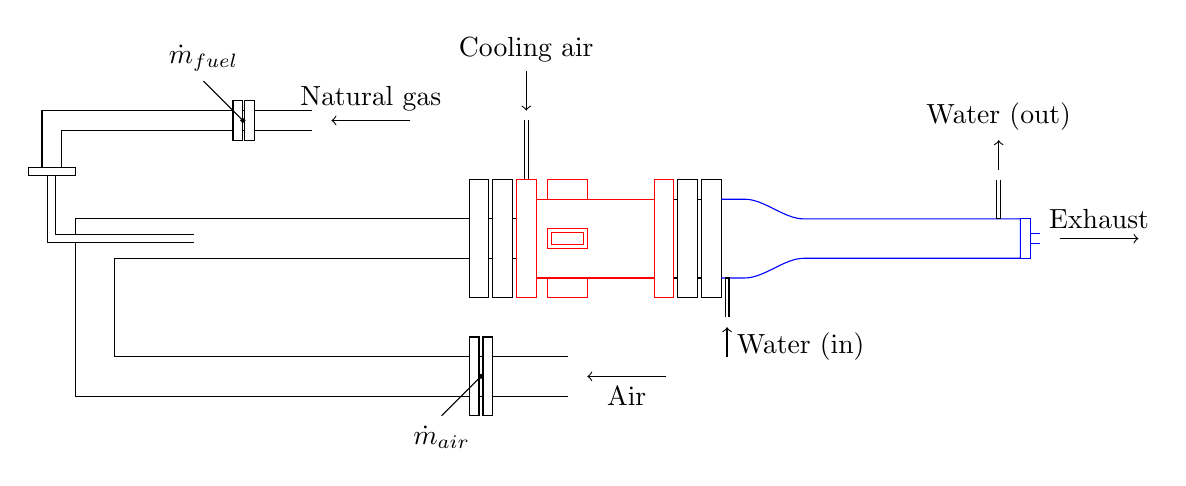
\begin{tikzpicture}[scale=0.5]

%% Air Supply
\draw ( -7, 0.1 ) -- ++( -3, 0 ) -- ++( 0, 0.4 ) -- ++( 10, 0 ) -- ++ ( 0, -1 ) -- ++ ( -9, 0 ) -- ++( 0, -2.5 ) -- ++ ( 9, 0 ) -- ++( 0, -1 ) -- ++( -10, 0 ) -- ++( 0, 3.9 ) -- ++( 3, 0 );
\draw ( 0, -4.5 ) rectangle +( 0.25, 2 );
\draw ( 0.25, -4 ) rectangle +( 0.1, 1 );
\draw ( 0.35, -4.5 ) rectangle +( 0.25, 2 );
\draw ( 0.6, -4 ) -- +( 1.9, 0 );
\draw ( 0.6, -3 ) -- +( 1.9, 0 );

%% Fuel Supply
\draw ( -10, 0.1 ) -- ++( -0.5, 0 ) -- ++( 0, 1.5 ) -- ++( -0.2, 0 ) -- ++( 0, -1.7 ) -- ++( 0.7, 0 );
\draw ( -10, 1.6 ) rectangle ++( -1.2, 0.2 );
\draw ( -10.35, 1.8 ) -- ++( 0, 0.95 ) -- ++( 4.35, 0 );
\draw ( -10.85, 1.8 ) -- ++( 0, 1.45 ) -- ++( 4.85, 0 );
\draw ( -6, 2.5 ) rectangle +( 0.25, 1 );
\draw ( -5.75, 2.75 ) rectangle +( 0.05, 0.5 );
\draw ( -5.7, 2.5 ) rectangle +( 0.25, 1 );
\draw ( -5.45, 2.75 ) -- +( 1.45, 0 );
\draw ( -5.45, 3.25 ) -- +( 1.45, 0 );

%% Cooling air supply
\draw ( 1.5, 3 ) -- ++( 0, -1.5 ) -- ++( -0.1, 0 ) -- ++( 0, 1.5 );

%% Pressure Vessel
% Upstream Flanges
\draw ( 0, -1.5 ) rectangle +( 0.5, 3 );
\draw ( 0.5, -0.5 ) rectangle +( 0.1, 1 );
\draw ( 0.6, -1.5 ) rectangle +( 0.5, 3 );
\draw ( 1.1, -0.5 ) rectangle +( 0.1, 1 );
\draw [red] ( 1.2, -1.5 ) rectangle +( 0.5, 3 );

% Vessel + Windows
\draw [red] ( 1.7, -1 ) rectangle +( 3, 2 );
\draw [red] ( 2, -1 ) rectangle +( 1, -0.5 );
\draw [red] ( 2, 1 ) rectangle +( 1, 0.5 );
\draw [red] ( 2, -0.25 ) rectangle +( 1, 0.5 );
\draw [red] ( 2.1, -0.15 ) rectangle +( 0.8, 0.3 );

% Downstream Flanges
\draw ( 5.9, -1.5 ) rectangle +( 0.5, 3 );
\draw ( 5.8, -1 ) rectangle +( 0.1, 2 );
\draw ( 5.3, -1.5 ) rectangle +( 0.5, 3 );
\draw ( 5.2, -1 ) rectangle +( 0.1, 2 );
\draw [red] ( 4.7, -1.5 ) rectangle +( 0.5, 3 );

%% Exhaust system
\draw [blue] ( 6.4, 1 ) -- ++( 0.6, 0 ) .. controls +( 0.5, 0 ) and +( -0.5, 0 ) .. ++( 1.5, -0.5 ) -- ++( 5.5, 0 ) -- ++( 0, -1 ) -- ++( -5.5, 0 ) .. controls +( -0.5, 0 ) and +( 0.5, 0 ) .. ++( -1.5, -0.5 ) -- ++ ( -0.6, 0 );
\draw [blue] ( 14, -0.5 ) rectangle ++( 0.25, 1 );
\draw [blue] (14.5, 0.125 ) -- ++( -0.25, 0 ) -- ++( 0, -0.25 ) -- ++( 0.25, 0 );

% Water cooling
\draw ( 6.5, -2 ) -- ++( 0, 1 ) -- ++( 0.1, 0 ) -- ++( 0, -1 );
\draw ( 13.5, 1.5 ) -- ++( 0, -1 ) -- ++( -0.1, 0 ) -- ++( 0, 1 );

%% Labels
\draw [->] ( 5, -3.5 ) -- ++( -2, 0 );
\node at ( 4, -3.5 ) [below] {Air};

\draw [->] ( -1.5, 3 ) -- ++( -2, 0 );
\node at ( -2.5, 3 ) [above] {Natural gas};

\draw [->] ( 1.45, 4.25 ) -- ++( 0, -1 );
\node at ( 1.45, 4.25 ) [above] {Cooling air};

\draw [->] ( 6.55, -3 ) -- ++( 0, 0.75 );
\node at ( 6.55, -2.75 ) [right] {Water (in)};

\draw [->] ( 13.45, 1.75 ) -- ++( 0, 0.75 );
\node at ( 13.45, 2.5 ) [above] {Water (out)};

\draw [->] ( 15, 0 ) -- ++( 2, 0 );
\node at ( 16, 0 ) [above] {Exhaust};

\filldraw ( -0.7, -4.5 ) node [below] {\(\dot{m}_{air}\)} -- ++( 1, 1 ) circle ( 0.05 );
\filldraw ( -6.75, 4 ) node [above] {\(\dot{m}_{fuel}\)} -- ++( 1, -1 ) circle ( 0.05 );

\end{tikzpicture}

\caption[Schematic of test facility A]{A schematic of the high pressure testing facility where Configuration A is operated is shown. The pressure vessel is outlined in \textcolor{red}{red}, while the water-cooled exhaust section is outlined in \textcolor{blue}{blue}. The locations of the orifice flow meters used to measure the mass flow rates of the preheated air and natural gas fuel are indicated.}

\label{fig:testFacilityA}

\end{figure}



Pressurized air is supplied from external tanks and heated in an indirect, gas-fired heat exchanger to about 500 K.
The flowrate of the air is metered using a sub-critical orifice flow meter with a 38 mm (1.5 in) bore diameter Flow-Lin orifice plate capable of metering a maximum flow rate of 2.2 kg/s (1 lb/s).
The orifice flow meter is instrumented with an Omega PX725A-1KGI pressure transmitter calibrated to a reduced pressure range of 0--2.758 MPa (0--400 psi), a shielded K-type thermocouple and an Omega PX771A-025GI differential pressure transmitter, calibrated to a reduced differential pressure range of 0--68.948 kPa (0--10 psid).
The fuel (natural gas) is metered using a similar set up as the air line, with a sub-critical orifice flow meter.
The orifice plate is a Flow-Lin orifice plate with a bore diameter of 13.46 mm (0.53 in), capable of metering a maximum flow rate of 0.22 kg/s (0.1 lb/s).
The upstream pressure is measured using an Omega PX725A-1KGI pressure transmitter (same as the air line) and the differential pressure is measured using a PX771A-100WDC differential pressure transmitter with a pressure range of 0--2.489 kPa (100 in \ce{H2O}).
The temperature of the fuel is assumed to be the same as the room temperature (300 K).

The air enters the inlet nozzle of the LSB through a 1.8 m (6 ft) long, 102 mm (4 in) diameter straight pipe section.
The straight pipe section allows for the flow to be fully developed, and fully premixed before the reactants enter the burner.
The combustor pressure and temperature are measured at the head of the inlet nozzle.
The pressure is measured by an Omega PX181B-500G5V pressure transducer with a pressure range of 0--3.45 MPa (0--500 psi), while the temperature is measured using a K-type thermocouple.

The pressure and temperature measurements are used to calculate the four primary flow parameters (combustor pressure, preheat temperature, reference velocity and equivalence ratio) for the LSB in real time.
All measurements are monitored and recorded during the course of the experiment by a LabView VI.

The pressure vessel enclosing the combustor is designed to withstand pressures of up to 30 atm and is insulated from the combustor by a ceramic liner.
Cooling for the pressure vessel and the quartz tube is provided by a flow of cold air introduced at the head of the pressure vessel.
The cold air is drawn from the same external tanks as the main air line, but bypassing the heating system.
The cold air flow is not metered, but its upstream pressure is coupled to the main air line so as to ensure a stead flow of cold air into the pressure vessel at all operating conditions.
Optical access to the combustor is provided through four 25 mm (1 in) thick, 150 mm (6 in)\(\times\)75 mm (3 in) quartz windows located \(90^\circ\) apart azimuthally.
The view ports allow the combustor to be imaged from the dump plane to an axial distance of 150 mm (6 in) downstream.

The exhaust from the combustor is cooled by circulating cold water through a water jacket enclosing each section of the exhaust pipe.
The length of the exhaust pipe sections is about 1.8 m (6 ft).
The exhaust pipe section terminates in an orifice plug to provide the back pressure to the combustion chamber.
Different diameter orifices are used for each reference velocity condition to be tested.
The exiting products are finally released to the building exhaust system.

\subsubsection{Low Swirl Burner}

\begin{figure}

\centering

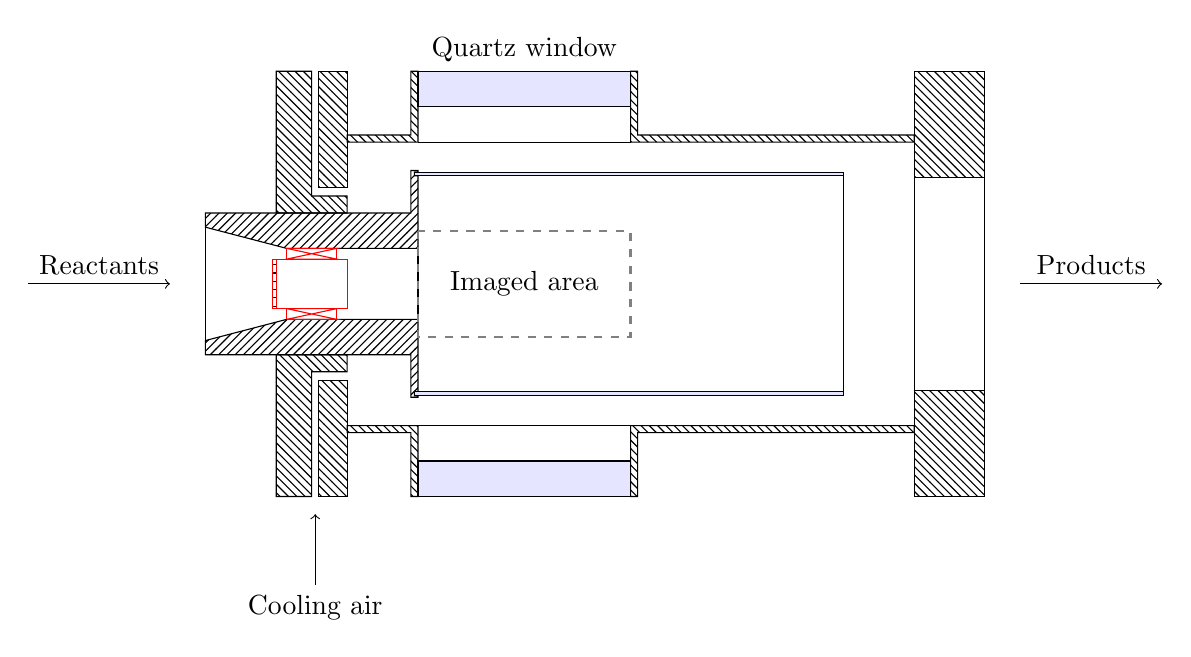
\begin{tikzpicture}[scale=0.9]

% Upstream flange
\draw[pattern=north west lines] ( 1, 1 ) -- ++( 1, 0 ) -- ++( 0, 0.24 ) -- ++( -0.5, 0 ) -- ++( 0, 1.76 ) -- ++( -0.5, 0 ) -- cycle;
\draw[pattern=north west lines] ( 2, 3 ) rectangle ++( -0.4, -1.64 );
\draw[pattern=north west lines] ( 1, -1 ) -- ++( 1, 0 ) -- ++( 0, -0.24 ) -- ++( -0.5, 0 ) -- ++( 0, -1.76 ) -- ++( -0.5, 0 ) -- cycle;
\draw[pattern=north west lines] ( 2, -3 ) rectangle ++( -0.4, 1.64 );

% Pressure vessel
\draw[pattern=north west lines] ( 2, 2 ) -- ++( 1, 0 ) -- ++( 0, 1 ) -- ++( -0.1, 0 ) -- ++( 0, -0.9 ) -- ++ ( -0.9, 0 ) -- cycle;
\draw ( 3, 2 ) -- ++( 3, 0 );
\draw[pattern=north west lines] ( 6, 2 ) -- ++( 4, 0 ) -- ++( 0, 0.1 ) -- ++( -3.9, 0 ) -- ++( 0, 0.9 ) -- ++( -0.1, 0 ) -- cycle;
\draw[pattern=north west lines] ( 2, -2 ) -- ++( 1, 0 ) -- ++( 0, -1 ) -- ++( -0.1, 0 ) -- ++( 0, 0.9 ) -- ++ ( -0.9, 0 ) -- cycle;
\draw ( 3, -2 ) -- ++( 3, 0 );
\draw[pattern=north west lines] ( 6, -2 ) -- ++( 4, 0 ) -- ++( 0, -0.1 ) -- ++( -3.9, 0 ) -- ++( 0, -0.9 ) -- ++( -0.1, 0 ) -- cycle;

% Quartz Windows
\draw[fill=blue!10!white] ( 3, 3 ) rectangle ++( 3, -0.5 );
\draw[fill=blue!10!white] ( 3, -3 ) rectangle ++( 3, 0.5 );

% Downstream flange
\draw [pattern=north west lines] ( 10, 1.5 ) rectangle ++( 1, 1.5 );
\draw [pattern=north west lines] ( 10, -1.5 ) rectangle ++( 1, -1.5 );
\draw ( 10, 1.5 ) -- ++( 0, -3 );
\draw ( 11, 1.5 ) -- ++( 0, -3 );

% Nozzle
\draw[pattern=north east lines] ( 0, 0.8 ) -- ++( 1.15, -0.3 ) -- ++( 1.85, 0 ) -- ++( 0, 1.025 ) -- ++( -0.05, 0 ) -- ++( 0, 0.05 ) -- ++( 0.05, 0 ) -- ++( 0, 0.025 ) -- ++ ( -0.1, 0 ) -- ++( 0, -0.6 ) -- ++( -2.9, 0 ) -- cycle;
\draw[pattern=north east lines] ( 0, -0.8 ) -- ++( 1.15, 0.3 ) -- ++( 1.85, 0 ) -- ++( 0, -1.025 ) -- ++( -0.05, 0 ) -- ++( 0, -0.05 ) -- ++( 0.05, 0 ) -- ++( 0, -0.025 ) -- ++ ( -0.1, 0 ) -- ++( 0, 0.6 ) -- ++( -2.9, 0 ) -- cycle;
\draw ( 0, 0.8 ) -- ++( 0, -1.6 );
\draw ( 3, 0.5 ) -- ++( 0, -1 );

% Swirler
\draw [red] ( 1.15, 0.5 ) -- ++( 0.7, 0 ) -- ++( -0.7, -0.15 ) -- ++( 0.7, 0 ) -- ++( -0.7, 0.15 ); 
\draw [red] ( 1.15, 0.5 ) -- ++( 0, -0.15 );
\draw [red] ( 1.85, 0.5 ) -- ++( 0, -0.15 );
\draw [red] ( 1, 0.35 ) rectangle ++( 1, -0.7 );
\draw [red] ( 1.15, -0.5 ) -- ++( 0.7, 0 ) -- ++( -0.7, 0.15 ) -- ++( 0.7, 0 ) -- ++( -0.7, -0.15 ); 
\draw [red] ( 1.15, -0.5 ) -- ++( 0, 0.15 );
\draw [red] ( 1.85, -0.5 ) -- ++( 0, 0.15 );
\draw[red,pattern=horizontal lines] ( 0.95, 0.35 ) rectangle ++( 0.05, -0.7 );

% Quartz tube
\draw[fill=blue!10!white] ( 2.95, 1.525 ) rectangle ++( 6.05, 0.05 );
\draw[fill=blue!10!white] ( 2.95, -1.525 ) rectangle ++( 6.05, -0.05 );
\draw ( 9, 1.525 ) -- ++( 0, -3.05 );

% Imaged region
\draw[thick,dashed,gray] ( 3, 0.75 ) rectangle ++( 3, -1.5 );

% Labels
\draw [->] ( -2.5, 0 ) -- ++( 2, 0 );
\node at ( -1.5, 0 ) [above] {Reactants};

\draw [->] ( 11.5, 0 ) -- ++( 2, 0 );
\node at ( 12.5, 0 ) [above] {Products};

\draw [->] ( 1.55, -4.25 ) -- ++( 0, 1 );
\node at ( 1.55, -4.25 ) [below] {Cooling air};

\node at ( 4.5, 3 ) [above] {Quartz window};
\node at ( 4.5, 0 ) {Imaged area};

\end{tikzpicture}

\caption[Detail schematic of Configuration A]{A cross-sectional view of Configuration A in the pressure vessel is shown. The reactants enter from the left. The products mix with the cooling air and leave on the right. The location of the swirler in the inlet nozzle is highlighted in \textcolor{red}{red}. Also shown is the region of the combustion zone that can be imaged through the quartz windows.}

\label{fig:lsbA}

\end{figure}



The detail of the LSB configuration is shown in Figure \ref{fig:lsbA}.
The premixed, preheated reactants reach the swirler through a converging nozzle that decreases linearly in diameter from from the inlet diameter of 102 mm (4 in) to the outer diameter of the swirler, 38 mm (1.5 in).
At the swirler, the flow splits into two streams---one passing through the central section and another picking up swirl by flowing over the vanes in the annular region.
The relative flow split between the two streams is controlled by inducing blockage into the central flow by means of a perforated plate.
The swirler leads to a constant area nozzle, and is located one diameter upstream of an abrupt area change.
At the area change, the reactants expand from the 38 mm (1.5 in) diameter nozzle into a 115 mm (4.5 in) diameter combustion zone.
This expansion ratio is chosen so as to avoid confinement effects on the centerline flame flow field.\cite{1998-yegian}

The main combustion zone begins at the dump plane and is enclosed by a GE 214 quartz tube.
The quartz tube is 300 mm (12 in) long and 115 mm (4.5 in) in diameter.
The thickness of the quartz tube is 2.5 mm (0.1 in).

\subsection{Configuration B}

This configuration was used to image the flame structure of the LSB flame using CH PLIF.
A schematic of the flow system of the test facility is shown in Figure \ref{fig:testFacilityB}, while the LSB combustor itself is shown in greater detail in Figure \ref{fig:lsbB}.

\subsubsection{Test Facility}

\begin{figure}

\centering

\begin{tikzpicture}

% Air Supply
\draw ( 2, -2.05 ) -- ++( -1.05, 0 ) -- ++( 0, 1.1 ) -- ++( 1, 0 ) -- ++( 0, 2.9 ) -- ++( -1.45, 0 );
\draw ( 2, -1.95 ) -- ++( -0.95, 0 ) -- ++( 0, 0.9 ) -- ++( 1, 0 ) -- ++( 0, 3.1 ) -- ++( -1, 0 ) -- ++( 0, 1 ) -- ++( -0.55, 0 );
\draw ( 0.5, 2.05 ) -- ++( 0.45, 0 ) -- ++( 0, 0.9 ) -- ++( -0.45, 0 );
\draw ( -0.5, 2.05 ) -- ++( -0.45, 0 ) -- ++( 0, 0.9 ) -- ++( 0.45, 0 );
\draw ( -0.5, 1.95 ) -- ++( -0.55, 0 ) -- ++( 0, 1.1 ) -- ++( 0.55, 0 );

\draw ( 2, -2.5 ) rectangle ++( 0.2, 1 );
\draw ( 2.2, -2.1 ) rectangle ++( 0.05, 0.2 );
\draw ( 2.25, -2.5 ) rectangle ++( 0.2, 1 );

\draw ( 2.45, -2.1 ) -- ++( 2.55, 0 ) -- ++( 0, -1.8 ) -- ++( -2.55, 0 );
\draw ( 2.45, -4.1 ) -- ++( 2.75, 0 ) -- ++( 0, 1 ) -- ++( 2.8, 0 );
\draw [red] ( 3.5, -2 ) circle ( 0.2 );
\draw [red] ( 3.5, -2 ) circle ( 0.175 );
\draw [red] ( 3.35, -2.1 ) -- ++( 0.3, 0.2 );
\draw [red] ( 3.35, -1.9 ) -- ++( 0.3, -0.2 );

\draw ( -0.1, 0 ) -- ++( 0, -4.1 ) -- ++( 2.1, 0 );
\draw ( 0.1, 0 ) -- ++( 0, -3.9 ) -- ++( 1.9, 0 );
\draw ( 2, -4.5 ) rectangle ++( 0.2, 1 );
\draw ( 2.2, -4.1 ) rectangle ++( 0.05, 0.2 );
\draw ( 2.25, -4.5 ) rectangle ++( 0.2, 1 );
\draw [red] ( 3.5, -4 ) circle ( 0.2 );
\draw [red] ( 3.5, -4 ) circle ( 0.175 );
\draw [red] ( 3.35, -4.1 ) -- ++( 0.3, 0.2 );
\draw [red] ( 3.35, -3.9 ) -- ++( 0.3, -0.2 );

% Fuel Supply
\draw ( 2.45, -1.9 ) -- ++( 2.75, 0 ) -- ++( 0, -1 ) -- ++( 0.8, 0 ) -- ++( 0, 0.95 ) -- ++( 1, 0 );
\draw ( 8, -2.9 ) -- ++( -1.9, 0 ) -- ++( 0, 0.85 ) -- ++( 0.9, 0 );
\draw ( 7, -2.25 ) rectangle ++( 0.1, 0.5 );
\draw ( 7.1, -2.05 ) rectangle ++( 0.025, 0.1 );
\draw ( 7.125, -2.25 ) rectangle ++( 0.1, 0.5 );
\draw ( 7.225, -2.05 ) -- ++( 0.775, 0 );
\draw ( 7.225, -1.95 ) -- ++( 0.775, 0 );

% Base flange
\draw ( -1.5, 0 ) rectangle ++( 3, 0.5 );

% Combustor
\draw ( -0.5, 0.5 ) -- ++( 0, 2.5 ) .. controls +( 0, 0.5 ) and +( 0, -0.5 ) .. ++( 0.35, 0.8 ) -- ++( 0.3, 0 );
\draw ( 0.5, 0.5 ) -- ++( 0, 2.5 ) .. controls +( 0, 0.5 ) and +( 0, -0.5 ) .. ++( -0.35, 0.8 );
\draw ( -0.15, 3.8 ) rectangle ++( 0.3, 0.7 );

% Labels
\draw [->] ( 9.5, -3 ) -- ++( -1.25, 0 );
\node at ( 9, -3 ) [below] {Air};

\draw [->] ( 9.5, -2 ) -- ++( -1.25, 0 );
\node at ( 9, -2 ) [above] {Natural gas};

\filldraw ( 2.225, -4 ) circle ( 0.05 ) -- ++( -0.5, -1 ) node [below] {\(\dot{m}_{core}\)};
\filldraw ( 2.225, -2 ) circle ( 0.05 ) -- ++( 0.5, 1 ) node [above] {\(\dot{m}_{swirl}\)};
\filldraw ( 7.1125, -2 ) circle ( 0.05 ) -- ++( 0.5, 1 ) node [above] {\(\dot{m}_{fuel}\)};

\end{tikzpicture}

\caption[Schematic of test facility B]{A schematic of the high pressure testing facility where Configuration B was operated is shown. The locations of the orifice flow meters on the reactant streams and fuel lines are shown. Valves (shown in \textcolor{red}{red}) on the swirl and core flow lines allow for the relative mass flow split to be varied between the two reactant streams. The upstream orifice flow meter on the preheated air line is not shown here. All preheated air lines are insulated.}

\label{fig:testFacilityB}

\end{figure}



This test facility shares the upstream supply of preheated air, cold air and fuel (natural gas) with the one used in Configuration A.
The flow rate of the preheated air stream is measured using the same orifice flow meter system used in Configuration A---albeit with a smaller 12.921 mm (0.5087 in) diameter bore Flow-Lin orifice plate.
The fuel system pressure is regulated from the building supply pressure to a lower required pressure by an adjustable TESCOM regulator and metered using a critical orifice flow meter.
The critical orifice on the fuel line has a bore diameter of 0.8128 mm (0.032 in).
The pressure upstream of the critical orifice is measured using an Omegadyne PX409-1.5KGI pressure transmitter with a range of 0--10.34 MPa (0--1500 psig) and the pressure downstream of the critical orifice is measured using a Dwyer 626 series pressure transmitter with a range of 0--3.45 MPa (0--500 psig).
The downstream pressure can be used to verify if the critical orifice is choked during operation.
The temperature of the fuel is measured upstream by a K-type thermocouple.

The air system is choked with a 5.41 mm (0.213 in) diameter critical orifice before mixing with the fuel.
A short distance after mixing, the reactants are split into two separate streams for the central flow and the swirl flow.
The central flow rate is measured using a 9.271 mm (0.365 in) diameter sub-critical orifice, instrumented with a Dwyer 626 series pressure transmitter with a range of 0--4.14 MPa (0--600 psig) for measuring the upstream pressure, a K-type thermocouple for measuring the upstream temperature and an Omega PX771-300WCDI differential pressure transducer with a range of 0--74.65 kPa (0--300 in \ce{H2O}).
The swirl flow rate is measured similarly, using a 11.68 mm (0.46 in) diameter sub-critical orifice, a Dwyer 626 series pressure transmitter with a range of 0--5.52 MPa (0--800 psig), a K-type thermocouple and another Omega PX771A-300WCDI with a differential pressure range of 0--74.65 kPa (0--300 in \ce{H2O}).
The relative flow split between the two reactant streams is controlled by partially closing gate valves on the two lines.

The cooling air flow line is choked, but not metered.
All measurements are monitored and recorded by a LabView VI.

The pressure vessel is rated for pressures in excess of 30 atm and is insulated from the combustor by a flow of cold air.
The cold air enters the pressure vessel through two inlet ports and passes through a layer of steel ball bearings which renders the flow uniform spatially.
The central and swirl flow reactant streams enter through separate ports and connect to the combustor.
The pressure vessel has four viewports located \(90^\circ\) apart for optical access.
Each viewport is covered by a 25 mm (1 in) thick, 178 mm (7 in) \(\times\) 50 mm (2 in) quartz window.
The LSB exit is located approximately halfway between the top and bottom edges of the window, allowing about 88.9 mm (3.5 in) of the combustion zone to be imaged through the window.
Similar to Test Rig A, the exhaust section is cooled by circulating cold water through an enclosing water jacket.
An adjustable gate valve on the exhaust line provides the back pressure necessary to pressurize the combustor.
The products are vented into the same building exhaust system as Configuration A.

\subsubsection{Low Swirl Burner}

\begin{figure}

\centering

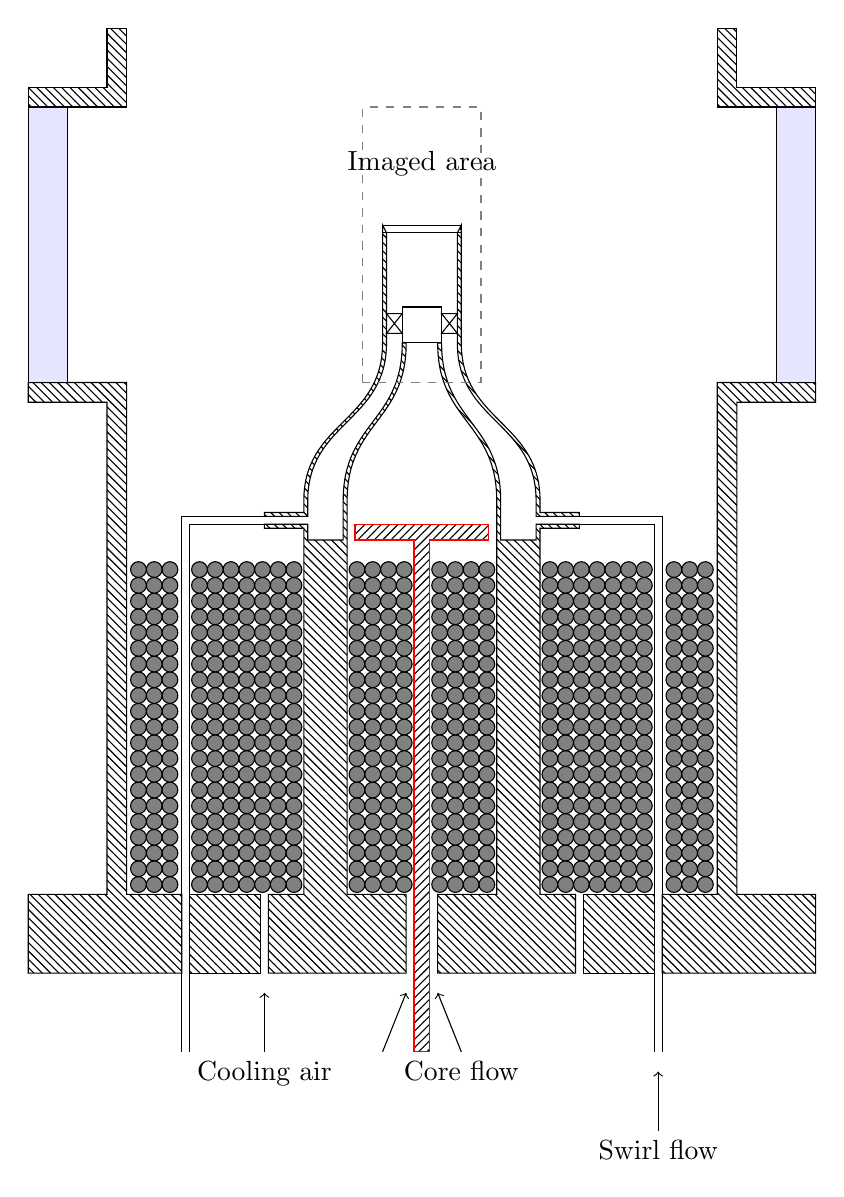
\begin{tikzpicture}

% Left half (lower)
\draw[pattern=north west lines] ( -1.5, 0 ) -- ++( 0, 4.65 ) -- ++( -0.5, 0 ) -- ++( 0, 0.05 ) -- ++( 0.55, 0 ) -- ++( 0, -0.2 ) -- ++( 0.45, 0 ) -- ++( 0, 0.5 ) .. controls +( 0, 1 ) and +( 0, -1 ) .. ++( 0.75, 2 ) -- ++( 0.05, 0 ) .. controls +( 0, -1 ) and +( 0, 1 ) .. ++( -0.75, -2 ) -- ++( 0, -5 ) -- ++( 0.75, 0 ) -- ++( 0, -1 ) -- ++( -1.75, 0 ) -- ++( 0, 1 ) -- cycle;

% Left half (upper)
\draw[pattern=north west lines] ( -2, 4.85 ) -- ++( 0.5, 0 ) -- ++( 0, 0.15 ) .. controls +( 0, 1 ) and +( 0, -1 ) .. ++( 1, 2 ) -- ++( 0, 1.5 ) -- ++( 0.05, -0.1 ) -- ++( 0, -1.4 ) .. controls +( 0, -1 ) and +( 0, 1 ) .. ++( -1, -2 ) -- ++( 0, -0.2 ) -- ++( -0.55, 0 ) -- cycle;

% Right half (lower)
\draw[pattern=north west lines] ( 1.5, 0 ) -- ++( 0, 4.65 ) -- ++( 0.5, 0 ) -- ++( 0, 0.05 ) -- ++( -0.55, 0 ) -- ++( 0, -0.2 ) -- ++( -0.45, 0 ) -- ++( 0, 0.5 ) .. controls +( 0, 1 ) and +( 0, -1 ) .. ++( -0.75, 2 ) -- ++( -0.05, 0 ) .. controls +( 0, -1 ) and +( 0, 1 ) .. ++( 0.75, -2 ) -- ++( 0, -5 ) -- ++( -0.75, 0 ) -- ++( 0, -1 ) -- ++( 1.75, 0 ) -- ++( 0, 1 ) -- cycle;

% Right half (upper)
\draw[pattern=north west lines] ( 2, 4.85 ) -- ++( -0.5, 0 ) -- ++( 0, 0.15 ) .. controls +( 0, 1 ) and +( 0, -1 ) .. ++( -1, 2 ) -- ++( 0, 1.5 ) -- ++( -0.05, -0.1 ) -- ++( 0, -1.4 ) .. controls +( 0, -1 ) and +( 0, 1 ) .. ++( 1, -2 ) -- ++( 0, -0.2 ) -- ++( 0.55, 0 ) -- cycle;

\draw ( -0.5, 8.5 ) -- ++( 1, 0 );
\draw ( -0.5, 8.4 ) -- ++( 1, 0 );

% Swirler
\draw ( -0.25, 7.01 ) rectangle ++( 0.5, 0.45 );
\draw ( -0.45, 7.125 ) -- ++( 0.2, 0.25 ) -- ++( -0.2, 0 ) -- ++( 0.2, -0.25 ) -- cycle;
\draw ( 0.45, 7.125 ) -- ++( -0.2, 0.25 ) -- ++( 0.2, 0 ) -- ++( -0.2, -0.25 ) -- cycle;

% Turbulence generator
\draw[red,pattern=north east lines] ( -0.1, -2 ) -- ++( 0, 6.5 ) -- ++( -0.75, 0 ) -- ++( 0, 0.2 ) -- ++( 1.7, 0 ) -- ++( 0, -0.2 ) -- ++( -0.75, 0 ) -- ++( 0, -6.5 ) -- cycle;

% Ball bearings (inside)
\foreach \x in { -0.825, -0.625, -0.425, -0.225 }
  \foreach \y in { 0.125, 0.325, ..., 4.125 }
    \draw[fill=black!50!white] ( \x, \y ) circle ( 0.1 );
\foreach \x in { 0.225, 0.425, 0.625, 0.825 }
  \foreach \y in { 0.125, 0.325, ..., 4.125 }
    \draw[fill=gray] ( \x, \y ) circle ( 0.1 );

% Ball bearings (outside)
\foreach \x in { -1.625, -1.825, ..., -2.825 }
  \foreach \y in { 0.125, 0.325, ..., 4.125 }
    \draw[fill=gray] ( \x, \y ) circle ( 0.1 );
\foreach \x in { 1.625, 1.825, ..., 2.825 }
  \foreach \y in { 0.125, 0.325, ..., 4.125 }
    \draw[fill=gray] ( \x, \y ) circle ( 0.1 );
\foreach \x in { -3.2, -3.4, -3.6 }
  \foreach \y in { 0.125, 0.325, ..., 4.125 }
    \draw[fill=gray] ( \x, \y ) circle ( 0.1 );
\foreach \x in { 3.2, 3.4, 3.6 }
  \foreach \y in { 0.125, 0.325, ..., 4.125 }
    \draw[fill=gray] ( \x, \y ) circle ( 0.1 );

% Upstream flange, Pressure vessel
\draw[pattern=north west lines] ( -2.05, -1 ) rectangle ++( -0.9, 1 );
\draw[pattern=north west lines] ( -3.05, 0 ) -- ++( -0.7, 0 ) -- ++( 0, 6.5 ) -- ++( -1.25, 0 ) -- ++( 0, -0.25 ) -- ++( 1, 0 ) -- ++( 0, -6.25 ) -- ++( -1, 0 ) -- ++( 0, -1 ) -- ++( 1.95, 0 ) -- cycle;

\draw[pattern=north west lines] ( 2.05, -1 ) rectangle ++( 0.9, 1 );
\draw[pattern=north west lines] ( 3.05, 0 ) -- ++( 0.7, 0 ) -- ++( 0, 6.5 ) -- ++( 1.25, 0 ) -- ++( 0, -0.25 ) -- ++( -1, 0 ) -- ++( 0, -6.25 ) -- ++( 1, 0 ) -- ++( 0, -1 ) -- ++( -1.95, 0 ) -- cycle;

\draw[pattern=north west lines] ( -5, 10 ) -- ++( 1.25, 0 ) -- ++( 0, 1 ) -- ++( -0.25, 0 ) -- ++( 0, -0.75 ) -- ++( -1, 0 ) -- cycle;
\draw[pattern=north west lines] ( 5, 10 ) -- ++( -1.25, 0 ) -- ++( 0, 1 ) -- ++( 0.25, 0 ) -- ++( 0, -0.75 ) -- ++( 1, 0 ) -- cycle;

% Quartz windows
\draw[fill=blue!10!white] ( 5, 6.5 ) rectangle ++( -0.5, 3.5 );
\draw[fill=blue!10!white] ( -5, 6.5 ) rectangle ++( 0.5, 3.5 );

% Swirl flow
\draw ( -2.95, -2 ) -- ++( 0, 6.7 ) -- ++( 0.95, 0 );
\draw ( -3.05, -2 ) -- ++( 0, 6.8 ) -- ++( 1.05, 0 );
\draw ( 2.95, -2 ) -- ++( 0, 6.7 ) -- ++( -0.95, 0 );
\draw ( 3.05, -2 ) -- ++( 0, 6.8 ) -- ++( -1.05, 0 );

% Imaged area
\draw [dashed, gray] ( -0.75, 6.5 ) rectangle ++( 1.5, 3.5 );

\draw [->] ( 0.5, -2 ) -- ++( -0.3, 0.75 );
\draw [->] ( -0.5, -2 ) -- ++( 0.3, 0.75 );
\node at ( 0.5, -2 ) [below] {Core flow};

\draw [->] ( 3, -3 ) -- ++( 0, 0.75 );
\node at ( 3, -3 ) [below] {Swirl flow};

\draw [->] ( -2, -2 ) -- ++( 0, 0.75 );
\node at ( -2, -2 ) [below] {Cooling air};

\node at ( 0, 9 ) [above] {Imaged area};

\end{tikzpicture}

\caption[Detail schematic of Configuration B]{A cross-sectional view of Configuration B in the pressure vessel is shown. The reactants enter from below in two separate streams (core flow and swirl flow), along with cooling air. Stainless steel ball bearings inside the plenum chamber and outside make the core flow and the cooling air flow spatially uniform. The turbulence generator is located within the plenum and is outlined in \textcolor{red}{red}.}

\label{fig:lsbB}

\end{figure}



The design of this LSB configuration is presented in Figure \ref{fig:lsbB}.
As described earlier, the reactants reach the LSB swirler device through two separate streams.
The core/central stream passes through a plenum chamber which is filled with steel ball bearings before approaching the swirler through a smoothly contoured nozzle with a high contraction ratio.
The annular/swirl stream reaches the swirler directly through a separate contoured nozzle.
The contraction ratio is chosen to inhibit the formation of thick boundary layers in the reactant streams.
The core stream passes through the central portion of the swirler, while the annular stream picks up swirl by passing through the vanes of the swirler.
The swirler lacks a perforated plate covering the central region as the primary function of the plate---regulating the relative mass flow split---is performed by the test facility itself.

The swirler device is located at the beginning of a constant area nozzle which is FIXME in length.
Following this, the reactants expand into the combustion zone.

Unlike in Configuration A, there is no dump plane or quartz tube to provide confinement to the combustion zone.
The co-flow of cold air provides insulation to the walls of the pressure vessel.
Also, as mentioned earlier, the relative mass flow split between the central and annular flows can be controlled directly.
Finally, the level of turbulence in the central flow can be adjusted by use of a turbulence generator\cite{2011-marshall} located upstream in the plenum chamber.

\section{Diagnostics}

\subsection{Laser Doppler Velocimetry}

\begin{figure}

\centering

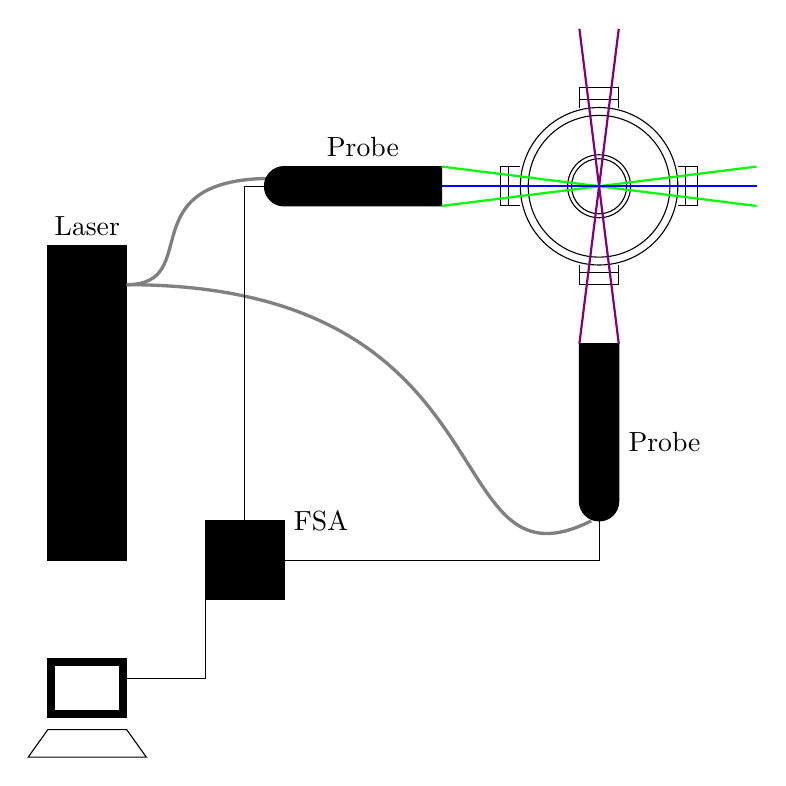
\begin{tikzpicture}

% Pressure vessel, quartz tube
\draw ( 6, 6.75 ) circle ( 1 );
\draw ( 6, 6.75 ) circle ( 0.9 );

\draw ( 5, 6.5 ) -- ++( -0.25, 0 ) -- ++( 0, 0.5 ) -- ++( 0.25, 0 );
\draw ( 5.75, 7.75 ) -- ++( 0, 0.25 ) -- ++( 0.5, 0 ) -- ++( 0, -0.25 );
\draw ( 7, 6.5 ) -- ++( 0.25, 0 ) -- ++( 0, 0.5 ) -- ++( -0.25, 0 );
\draw ( 5.75, 5.75 ) -- ++( 0, -0.25 ) -- ++( 0.5, 0 ) -- ++( 0, 0.25 );

\draw ( 4.85, 6.5 ) -- ++( 0, 0.5 );
\draw ( 5.75, 7.85 ) -- ++( 0.5, 0 );
\draw ( 7.1, 6.5 ) -- ++( 0, 0.5 );
\draw ( 5.75, 5.65 ) -- ++( 0.5, 0 );

\draw ( 6, 6.75 ) circle ( 0.4 );
\draw ( 6, 6.75 ) circle ( 0.35 );

% Laser
\filldraw ( -1, 2 ) rectangle ++( 1, 4 );

% Fiber optic cables
\draw [very thick, gray] ( 0, 5.5 ) .. controls +( 1, 0 ) and +( -1.85, 0 ) .. ++( 1.85, 1.35 );
\draw [very thick, gray] ( 0, 5.5 ) .. controls +( 5, 0 ) and +( -2, -1 ) .. ++( 5.9, -3 );

% Probe A
\filldraw [black] ( 4, 7 ) -- ++( 0, -0.5 ) -- ++( -2, 0 ) arc ( 270:90:0.25 ) -- cycle;

\draw ( 1.75, 6.75 ) -- ++( -0.25, 0 ) -- ++( 0, -4.25 );

% Probe B
\filldraw [black] ( 5.75, 4.75 ) -- ++( 0.5, 0 ) -- ++( 0, -2 ) arc ( 0:-180:0.25 ) -- cycle;

\draw ( 6, 2.5 ) -- ++( 0, -0.5 ) -- ++( -4, 0 );

% Laser beams
\draw[green,thick] ( 4, 7 ) -- ++( 4, -0.5 );
\draw[green,thick] ( 4, 6.5 ) -- ++( 4, 0.5 );
\draw[blue,thick] ( 4, 6.75 ) -- ++( 4, 0 );
\draw[violet,thick] ( 5.75, 4.75 ) -- ++( 0.5, 4 );
\draw[violet,thick] ( 6.25, 4.75 ) -- ++( -0.5, 4 ) ;

% FSA
\filldraw [black] ( 1, 1.5 ) rectangle ++( 1, 1 );

% Computer
\filldraw [black] ( -1, 0 ) rectangle ++( 1, 0.75 );
\filldraw [white]( -0.9, 0.1 ) rectangle ++( 0.8, 0.55 );
\draw ( -1, -0.15 ) -- ++( 1, 0 ) -- ++( 0.25, -0.35 ) -- ++( -1.5, 0 ) -- cycle;

\draw ( 0, 0.5 ) -- ++( 1, 0 ) -- ++( 0, 1 );

% Labels
\node at ( -0.5, 6 ) [above] {Laser};
\node at ( 2, 2.5 ) [right] {FSA};
\node at ( 6.25, 3.5 ) [right] {Probe};
\node at ( 3, 7.25 ) {Probe};

\end{tikzpicture}

\caption[Schematic of the LDV setup]{The schematic shows the setup employed to map the velocity field of the LSB combustor using Laser Doppler Velocimetry. Three pairs of orthogonal beams are separated from the Argon Ion Laser output and conveyed by fiber optic cables (\textcolor{gray}{gray}) to optical probes mounted 90\(^\circ\) apart about the axis of the LSB combustor. The \textcolor{green}{green}, \textcolor{blue}{blue}, and \textcolor{violet}{violet} beams in the schematic represent the 514 nm, 488 nm and 476 nm wavelengths. The signal is collected by the transceiver probes and analyzed by the FSA module. The results are saved for further analysis.}

\label{fig:ldvSetup}

\end{figure}



The velocity field of the LSB is mapped using a TSI 3-component LDV system.
Three wavelengths (514 nm, 488 nm and 476 nm) are separated from the output of a 5 W Argon ion laser by an FBL-3 multicolor beam generator.
The individual beams are split into two coherent beams which are then focused to intersect and produce interference fringes within an ellipsoidal measurement volume with dimensions of the order of 100 \(\mu\)m.
For this purpose, two transceiver probes are mounted \(90^\circ\) apart about the axis of the LSB.
The setup is illustrated as a schematic in Figure \ref{fig:ldvSetup}.
One transceiver probe focuses the 514 nm and 488 nm beams in planes perpendicular to each other, while the second probe focuses the 476 nm beams orthogonal to the other two beams.
Particles in the flow field crossing the interference fringes scatter the laser light elastically and produce a sinusoidal signal whose frequency is proportional to the velocity of the particle.
The transceiver probes collect this scattered light and each wavelength is detected separately by a PDM-1000-3 three-channel photodetector module.
The output from the photodetector is processed by an FSA-3500-3 signal processor.
The resulting three components of the particle/flow velocity are recorded by the FlowSizer software.

Since the airflow is very sparsely populated by particles, the flow needs to be artificially seeded to facilitate LDV measurements in a reasonable amount of time.
The seeding particles to be used and their mean diameter are decided by the characteristics of the flow to be imaged.\cite{1997-melling}
Since the LSB flow field is a reacting one, the particles need to have high melting points.
Further, the particles need to be small enough to follow the flow closely and large enough or reflective enough to scatter light efficiently in the measurement volume.
Based on these requirements, commercially available alumina particles with a mean particle diameter of 5 \(\mu\)m were chosen for this study.
In order to uniformly seed the flow, a novel seeding generator was designed as described in Appendix \ref{app:seeder}.
The seeding particles were introduced slightly upstream of the 1.8 m (6 ft) long straight pipe section in Test Rig A.

LDV data was only acquired at atmospheric pressure conditions.
At high pressure conditions, the reacting LSB flow field produces sharp refractive index gradients that rapidly shift in the turbulent flow field.
This causes strong beam steering effects making it very difficult for the laser beams to reliably intersect within such a small measurement volume.
The long distance traveled by the beams in the test rig further exacerbated this problem, making LDV data nearly impossible to acquire at such conditions.

\subsection{CH* chemiluminescence}
\label{sec:chemiluminescence}

The LSB flame is imaged using one of two 16-bit intensified CCD cameras---PI Acton 1024\(\times\)256 or 512\(\times\)512 pixels---with a 28 mm f/2.8 camera lens.
CH* chemiluminescence is filtered using a bandpass filter centered on 430 nm with a FWHM of 10 nm.
At each operating condition, 100 instantaneous images are acquired with an exposure of 1 ms.
An additional 100 instantaneous images are acquired with no flame and averaged to yield the background for correcting the flame images.

CH* chemiluminescence has several advantages over flame chemiluminescence from other radicals such as OH*, \ce{C2}*, etc.
First, the CH* emission occurs around 430 nm and is less affected by blackbody radiation from the walls of the combustor compared to longer wavelength detection, e.g., \ce{C2}*, which emits around 514 nm.
Second, the intensity of the chemiluminescence from CH* is known to scale well with heat release in the combustor\cite{2006-hardalupas}, unlike \ce{C2}*.
Third, the emitted light can be gathered with high quantum efficiency by the intensified CCD cameras available for this study.
Particularly, the quantum efficiency of the 18 mm Gen III HB filmless intensifier used by the 512\(\times\)512 camera is about 45\% at 430 nm, compared to about 10\% at 310 nm, where OH* chemiluminescence peaks.

\subsubsection{Image Processing}

\begin{figure}

\centering

\begin{subfigure}{\linewidth}
  \centering
  \input{figures/sampleAverageImage}
%  \vspace{-20pt}
  \caption{Average CH* chemiluminescence image}
  \label{fig:sampleAverageImage}
\end{subfigure}

\begin{subfigure}{\linewidth}
  \centering
  \input{figures/sampleCenterlineIntensity}
  \caption{Centerline CH* chemiluminescence intensity}
  \label{fig:sampleCenterlineIntensity}
\end{subfigure}

\begin{subfigure}{\linewidth}
  \centering
  \input{figures/sampleAbelImage}
  \caption{Abel deconvoluted half-image}
  \label{fig:sampleAbelImage}
\end{subfigure}

\caption[Sample CH* Chemiluminescence data]{These images illustrate the processing of a typical CH* chemiluminescence dataset. The top image is the mean of 100 frames and shows the LSB flame at 9 atm. The flame standoff distance is calculated by locating the inflection point in the smoothed intensity profile (middle). An Abel deconvolution (bottom) can be used to highlight the flame brush and measure the angle of the flame.}

\label{fig:sampleFlameImages}

\end{figure}



The flame chemiluminescence images acquired are background-corrected and averaged.
The resulting mean is the line-of-sight integrated, time-averaged image of the flame.
Strictly speaking, this is not the same as a real average obtained from a long exposure image as the instantaneous images are obtained through a periodic sampling process and hence, are prone to statistical errors.
However, the behaviour of the flame can be assumed to be sufficiently random that the mean obtained is adequately representative of the true average.
Figure \ref{fig:sampleAverageImage} shows a typical mean CH* chemiluminescence image prepared in this manner.

Even when background-corrected, the walls of the combustor are not at zero intensity in the average chemiluminescence image.
This is particularly noticeable near the dump plane where there is no flame present and yet the walls are clearly illuminated.
The source of this background illumination is mostly the chemiluminescence from the flame scattering off the combustor and pressure vessel walls.
The contribution from blackbody radiation from the heated walls is less significant in the narrow wavelength range imaged.
This is evident from images acquired immediately after a flame blowout which show the walls to be nearly dark.

The averaged chemiluminescence image allows us to measure the flame standoff distance by following the intensity profile along the centerline of the combustor.
The intensity profile rises sharply when passing the flame standoff location.
Thus, the flame standoff location can be ascertained by finding the inflection point in the intensity profile.

The profile of the average chemiluminescence intensity along the centerline of the sample case from Figure \ref{fig:sampleAverageImage} is shown in Figure \ref{fig:sampleCenterlineIntensity}, showing the flame standoff distance.
The distance from the dump plane, measured in number of pixels on the image and scaled by the appropriate magnification factor yields the flame standoff distance, \(X_f\).
The determination of the flame standoff location by this method provides a suitable and deterministic means to locating the leading edge of the flame front.
\nomenclature{\(X_f\)}{Flame standoff distance}

The average image can be processed further to yield more spatially resolved information about the flame brush.
Under the reasonable assumption that the average LSB flame is axially symmetric about the centerline of the combustor, a tomographic deconvolution technique called an Abel deconvolution\cite{1992-dasch} can be used to convert the line-of-sight integrated image to a radial map of chemiluminescence intensity.
In effect, this shows the shape and structure of the average flame brush.
The Abel deconvolution of the sample data from Figure \ref{fig:sampleAverageImage} is shown in Figure \ref{fig:sampleAbelImage}.

The Abel-deconvoluted image provides an relatively easy means to determining the angle of the flame brush.
A straight line joining two points located at the center of the flame brush intersects the axis of the combustor at this angle.
The angle of the flame is denoted by \(\theta_f\).

Using the Abel deconvolution to study the flame brush suffers from two main drawbacks.
First, the system of equations describing the Abel deconvolution is only valid as long as the entirety of the flame is visible.
This is only satisfied in the initial region of the LSB where the diameter of the flame brush is smaller than the height of the optical viewport.
At further downstream locations, the flame is not imaged in its entirety.
This causes the spurious bright regions near the top of the window in Figure \ref{fig:sampleAbelImage}.
The second limitation of the Abel deconvolution technique stems from the high incidence of errors along the centerline (where \(r \to 0\)).
Due to this, any study of the flame brush thickness at the flame stabilization point---a metric of considerable importance---is all but impossible using this tomographic technique.

\subsection{CH Planar Laser-Induced Fluorescence}

\begin{figure}

\centering

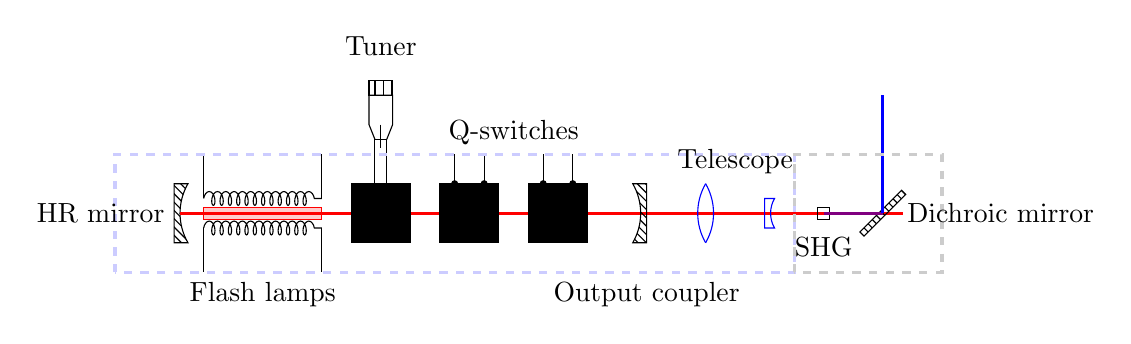
\begin{tikzpicture}[scale=0.75]

% HR reflector
\draw [pattern=north west lines] ( 0.1, 0 ) arc ( 180 : 210 : 1 ) -| ( 0, 0 );
\draw [pattern=north west lines] ( 0.1, 0 ) arc ( 180 : 150 : 1 ) -| ( 0, 0 );

% Active medium
\filldraw [red!20!white, draw=red] ( 0.5, -0.1 ) rectangle ++( 2, 0.2 );

% Main Beam
\draw [very thick,red] ( 0.1, 0 ) -- ++( 12.25, 0 );

% Flash lamps
\draw ( 0.5, 0.25 ) -- ++( 0, 0.75 );
\draw ( 2.5, 0.25 ) -- ++( 0, 0.75 );
\draw[decorate, decoration={coil,segment length=3}] ( 0.5, 0.25 ) -- ++( 2, 0 );

\draw ( 0.5, -0.25 ) -- ++( 0, -0.75 );
\draw ( 2.5, -0.25 ) -- ++( 0, -0.75 );
\draw[decorate, decoration={coil,segment length=3}] ( 0.5, -0.25 ) -- ++( 2, 0 );

% Birefringent tuner
\filldraw [black] ( 3, -0.5 ) rectangle ++( 1, 1 );
\draw ( 3.4, 0.5 ) rectangle ++( 0.2, 0.75 );
\draw ( 3.4, 1.25 ) -- ++( -0.1, 0.25 ) -- ++( 0, 0.5 ) -- ++( 0.4, 0 ) -- ++( 0, -0.5 ) -- ++( -0.1, -0.25 );
\draw [pattern=vertical lines] ( 3.3, 2 ) rectangle ++( 0.4, 0.25 );
\draw ( 3.5, 1.5 ) -- ++( 0, -0.4 );

% Qswitch 1
\filldraw [black] ( 4.5, -0.5 ) rectangle ++( 1, 1 );
\filldraw [black] ( 4.75, 0.5 ) circle ( 0.05 );
\filldraw [black] ( 5.25, 0.5 ) circle ( 0.05 );
\draw ( 4.75, 1 ) -- ++( 0, -0.5 );
\draw ( 5.25, 1 ) -- ++( 0, -0.5 );

% Q-switch 2
\filldraw [black] ( 6, -0.5 ) rectangle ++( 1, 1 );
\filldraw [black] ( 6.25, 0.5 ) circle ( 0.05 );
\filldraw [black] ( 6.75, 0.5 ) circle ( 0.05 );
\draw ( 6.25, 1 ) -- ++( 0, -0.5 );
\draw ( 6.75, 1 ) -- ++( 0, -0.5 );

% Output coupler
\draw [pattern=north west lines] ( 7.9, 0 ) arc ( 0 : 30 : 1 ) -| ( 8 , 0 );
\draw [pattern=north west lines] ( 7.9, 0 ) arc ( 0 : -30 : 1 ) -| ( 8, 0 );

% Converging lens
\draw [blue] ( 9, 0.5 ) arc ( 30 : -30 : 1 );
\draw [blue] ( 9, 0.5 ) arc ( 150: 210 : 1 );

% Diverging lens
\draw [blue] ( 10.1, 0 ) arc ( 180 : 210 : 0.5 ) -| ( 10, 0 );
\draw [blue] ( 10.1, 0 ) arc ( 180 : 150 : 0.5 ) -| ( 10, 0 );

% Doubling crystal
\draw ( 10.9, -0.1 ) rectangle ++( 0.2, 0.2 );

% Dichroic mirror
\draw [rotate around={45:( 12, 0 )},pattern=north west lines] ( 11.5, -0.05 ) rectangle ++( 1, 0.1 );

% SHG Beam
\draw [very thick, red!50!blue] ( 11, 0 ) -- ++( 1, 0 );
\draw [very thick, blue] ( 12, 0 ) -- ++( 0, 2 );

% Housing
\draw [dashed, very thick, blue!20!white] ( -1, -1 ) rectangle ++( 11.5, 2 );
\draw [dashed, very thick, black!20!white] ( 10.5, -1 ) rectangle ++( 2.5, 2 );

% Labels
\node at ( 0, 0 ) [left] {HR mirror};
\node at ( 1.5, -1 ) [below] {Flash lamps};
\node at ( 3.5, 2.5 ) [above] {Tuner};
\node at ( 5.75, 1 ) [above] {Q-switches};
\node at ( 8, -1 ) [below] {Output coupler};
\node at ( 9.5, 0.5 ) [above] {Telescope};
\node at ( 11, -0.25 ) [below] {SHG};
\node at ( 12.25, 0 ) [right] {Dichroic mirror};

\end{tikzpicture}

\caption[Schematic of the Alexandrite laser]{A schematic of the components of the PAL 101 Alexandrite laser is shown. The resonator formed by a High Reflection (HR) mirror and an output coupler is built around an alexandrite rod (\textcolor{red}{red}) pumped by flashlamps. The frequency of the output is selected by a tuner mechanism. Only one of the two Q-switches was used for this study. The laser beam is reduced in diameter by a collimating telescope (\textcolor{blue}{blue}) before passing through the Second Harmonic Generator (SHG). The UV beam is separated from the fundamental by a dichroic mirror and exits the laser. The fundamental beam terminates within the laser in a beam dump.}

\label{fig:laser}

\end{figure}



The CH PLIF setup uses the frequency-doubled output of a Light Age PAL 101 alexandrite laser tuned to \(\lambda \approx 387.2\) nm.
The design of the laser is shown schematically in Figure \ref{fig:laser}.
The active medium is a 150 mm (6 in) long, 5 mm (0.197 in) diameter alexandrite rod.
The rod is placed between two flashlamps within the resonator cavity formed by two spherical mirrors.
A birefringent tuning mechanism is placed within the resonator to allow the user to select the frequency of the output beam.
The tuning mechanism is coupled to a micrometer whose reading relates linearly to the output wavelength.
The tuning mechanism allows the fundamental wavelength to be varied between 720--780 nm, with peak gain at about 755 nm.
The resonator cavity also contains two Q-switches, which allow the laser to optionally operate in double-pulsed mode.
For this study, however, only one Q-switch was used and the laser was operated in single-pulsed mode only.

The diameter of the fundamental beam exiting the output coupler is reduced by a collimating telescope.
This is done in order to increase the efficiency of conversion of the frequency-doubling crystal.
The second harmonic portion of the beam is separated from the fundamental by a dichroic mirror and exits the laser.
The fundamental beam is terminated at a beam dump within the laser.

The alexandrite laser is capable of operating at frequencies of up to 15 Hz.
Laser power is controlled primarily by varying the voltage applied to the flash lamps.
When operating with a high flash lamp voltage, it is recommended that the frequency of pulsing be reduced to allow more time to dissipate the heat build up within the alexandrite rod.
All experiments conducted as part of this study operated the laser at 10.0 Hz.

The linewidth of the fundamental beam is determined by the manufacturer to be 150 GHz at \(\lambda\) = 775 nm.
Assuming the spectral profile of the laser to be a Gaussian, the linewidth of the frequency-doubled beam can be determined.
The Full Width at Half Max (FWHM) of a Gaussian curve scales linearly with the standard deviation of the curve.
When convoluted with itself, the new standard deviation is \(\sqrt{\sigma^2 + \sigma^2}\) or \(\sqrt{2}\) times that of the original curve.
Thus, the new linewidth is 150 \(\times\sqrt{2}\) = 212 GHz or 7.07 cm\(^{-1}\).
In wavelengths, this represents a spread of about 1.06 \AA.

\subsubsection{Imaging system}
\label{sec:imagingsystem}

All LIF imaging is performed with an intensified PI Acton 512\(\times\)512 camera.
The intensified camera is equipped with an 18 mm Gen III HB filmless intensifier with a quantum efficiency of about 45\% in the 420--440 nm range.
The lens is chosen depending on imaging requirements of each experiment.
In all cases, elastic scattering from the laser beam is attenuated by a 3 mm thick GG 420 Schott Glass filter.

\subsubsection{Laminar Flame setup}
\label{sec:laminarflamesetup}

Preliminary experiments to evaluate the CH PLIF technique are performed on a laminar flame.
The choice of a laminar flame as the subject allows us to neglect effects of strain and turbulence on the flame.
Further, laminar flames are more readily simulated by reaction kinetics packages like Chemkin with high fidelity.

These experiments are conducted on an laminar, methane-air flame stabilized on an unpiloted Bunsen burner with an inner diameter of 10.16 mm (0.4 in).
The air flow rate was measured and regulated using a Dwyer rotameter with a range of 0--20 SCFH calibrated using a Ritter drum-type gas meter.
The natural gas flow rate was metered using a Matheson FM 1050 602 rotameter with a range from 0--1230 SCCM.
This flowmeter was calibrated using a Sensidyne Gilibrator 2 bubble flow meter system.

\subsubsection{Laser Wavelength Calibration}

\begin{figure}

\centering

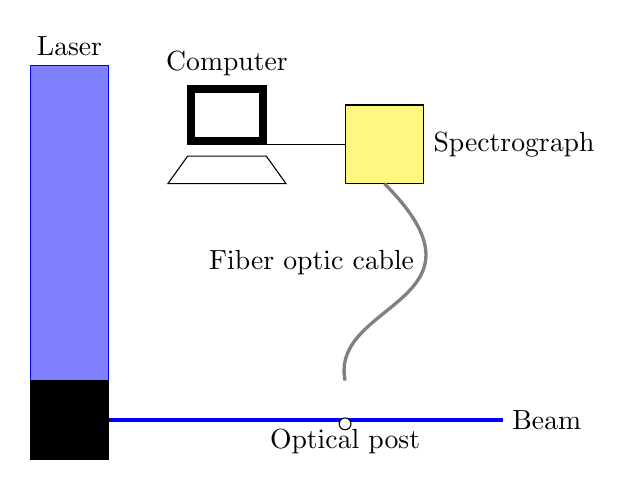
\begin{tikzpicture}

% Laser
\filldraw [fill=blue!50!white, draw=blue] ( 0, 5 ) rectangle ++( 1, -4 );
\filldraw [black] ( 0, 1 ) rectangle ++( 1, -1 );

% Beam
\draw [very thick, blue] ( 1, 0.5 ) -- ++( 5, 0 );

% Optical post
\filldraw [fill=white, draw=black] ( 4, 0.45 ) circle ( 0.075 );
% Computer
\filldraw [black] ( 2, 4 ) rectangle ++( 1, 0.75 );
\filldraw [white]( 2.1, 4.1 ) rectangle ++( 0.8, 0.55 );
\draw ( 2, 3.85 ) -- ++( 1, 0 ) -- ++( 0.25, -0.35 ) -- ++( -1.5, 0 ) -- cycle;

\draw ( 3, 4 ) -- ++( 1, 0 );

% Spectrometer
\filldraw [fill=yellow!50!white, draw=black] ( 4, 3.5 ) rectangle ++( 1, 1 );

% Optical fiber
\draw [very thick, gray] ( 4.5, 3.5 ) .. controls +( 1.5, -1.5 ) and +( -0.2, 1 ) .. ++( -0.5, -2.5 );

% Labels
\node at ( 0.5, 5 ) [above] {Laser};
\node at ( 2.5, 4.75 ) [above] {Computer};
\node at ( 5, 4 ) [right] {Spectrograph};
\node at ( 5, 2.5 ) [left] {Fiber optic cable};
\node at ( 4, 0.5 ) [below] {Optical post};
\node at ( 6, 0.5 ) [right] {Beam};

\end{tikzpicture}

\caption[Schematic of the laser calibration experiment]{The figure above shows the schematic of the experiment performed to calibrate the wavelength of the laser output. The laser output (containing mostly UV, but also a small portion of the fundamental frequency) is glanced off a steel optical post. The scattered light is gathered by a fiber optic cable (\textcolor{gray}{gray}) and sent to a spectrometer. The spectrum is analyzed to track the location of the fundamental frequency with tuner position. The UV peak is not tracked as the spectrometer is not calibrated for that wavelength.}

\label{fig:laserCalibration}

\end{figure}



As described earlier, the output wavelength of the PAL 101 alexandrite laser is controlled using a micrometer-coupled birefringent tuning mechanism.
The wavelength of the laser beam varies linearly with the micrometer reading.
Initially, the manufacturer-supplied calibration for the micrometer was found to be inaccurate.
This required an experiment to calibrate the laser output wavelength against the micrometer reading in order to determine the slope and offset of the calibration curve accurately.

A schematic of this experiment is shown in Figure \ref{fig:laserCalibration}.
The laser beam is glanced off a steel optical post and the scattered light is collected using a fiber-optic cable coupled to an Ocean Optics HR 2000 spectrometer.
The spectrometer is pre-calibrated using 50 wavelengths in the 400--850 nm range from the output of a Neon discharge lamp source.
The spectrometer is also intensity corrected over this range using a black body source.
The estimated error in the resolution of the device is about 0.1 nm (1 \AA).

The laser micrometer was traversed from 0.600 in to 0.625 in in steps of 0.001 in.
The experiment is repeated by traversing the micrometer from 0.625 in back to 0.600 in along the same points to ensure repeatability and estimate the variation due to hysteresis.
The calibration was performed using at the fundamental wavelength of the laser.
Each spectrum recorded is integrated over 512 ms and averaged over 10 such acquisitions.
The background-corrected peak of the spectrum is then modeled as a Gaussian and the location of the center of the Gaussian waveform is recorded.

\begin{figure}

\centering

\input{figures/laserCalibrationResultsPlot}

\caption[Laser wavelength calibration chart]{The wavelength of the second harmonic beam of the laser is plotted above against the tuner position(\(x\)). The data shows excellent repeatability and falls on a linear trend. The equation for the linear curve fit is \(\lambda = 330.213 + 91.5908x\), where the units of \(\lambda\) and \(x\) are nm and in, respectively.}

\label{fig:laserCalibrationResults}

\end{figure}



The results from this experiment are shown in Figure \ref{fig:laserCalibrationResults}.
The plot shows that the variation of the second harmonic wavelength (obtained by halving the fundamental wavelength) with the position of the tuner micrometer is verifiably linear.
Further, there is little difference between the measurements taken while increasing and decreasing the micrometer position.
This indicates that any effects of hysteresis in the micrometer position are minimal.
The calibration equation is obtained by applying a linear curve fit to the data points on the graph.


\chapter{CH PLIF Signal Modeling and Validation}

% This chapter covers the modeling of the CH PLIF signal and contains the following sections:

% 1. Signal modeling
%     1.1 Quenching models
% 2. Methane + air flames
%     2.1 subsection comparison with experiments
% 3. C1-C3 alkanes flames
% 4. Syngas mixtures
% 5. Syngas + C1-C3 alkanes
% 6. Effect of strain

% Questions to be answered (from proposal):

% 1. Detailing the development of a CH PLIF system (covered in Chapter 2,3 and here)
% 2. Demonstration on an atmospheric pressure laminar flame
% 3. Validate with quenching models
% 4. Model signal for strained flames
% 5. Model signal for fuel mixtures

\section{Fluorescence Signal Intensity}

As described in Chapter FIXME 2, the excitation scheme used in this study produces fluorescence through a three-step process.
First, the CH radicals in the ground state \(X^2\Pi, v=0\) are excited by the incident radiation to the second electronically excited state \(B^2\Sigma^-, v=0\).
This excitation occurs near the R-bandhead and targets the ground state CH radicals present in the rotational energy levels, \(N=5\) through 9.
The upper electronic state \(B^2\Sigma^-, v=0\) is nearly degenerate with the \(A^2\Delta, v=1\) energy level.
This leads to the population of the \(A^2\Delta, v=0,1\) energy levels due to collisional energy transfer.
The resulting fluorescence collected is primarily the result of three spontaneous transitions --- \(A\rightarrow X(1,1)\), \(A\rightarrow X(0,0)\) and \(B\rightarrow X(0,1)\).
These transitions are shown in Figure FIXME.

The primary goal of this exercise of modeling the CH fluorescence signal intensity is to gage the feasibility of using CH PLIF to study various premixed flames, rather than to quantitatively calculate the amount of CH present in the flames.
As such, we are more interested in the order of magnitude of the PLIF signal, rather than the absolute value of it.

The intensity of the CH fluorescence signal may be written as a function of the amount of CH radicals present in the excited state and the probability of spontaneous emission from said state.
Symbolically, this may be written as shown in Equation \ref{eqn:signalIntensity}.

\begin{equation}
S=nVA
\label{eqn:signalIntensity}
\end{equation}

In Equation \ref{eqn:signalIntensity}, \(S\) is the total number of photons emitted per unit time, \(n\) is the number of excited CH radicals in a unit volume, \(V\) is the volume from which the signal is observed.
The Einstein coefficient for spontaneous emission, \(A\) represents the probability of spontaneous emission between the two involved energy states.
The predicted signal intensity represents the total number of photons emitted in all directions.
In reality, only a fraction of these emitted photons will be recorded by the collection system.
This fraction is a function of the experimental setup and depends on the collection angle, the efficiency of the optics and the detector used to record the signal.
This fraction is left out because our objective is only to predict the relative variation in the signal between various premixed flames.

This formulation of the signal intensity implicitly makes the following assumptions.
\begin{enumerate}
\item The fluorescence emission is predicted at steady state.
\item The collection volume is optically thin and an emitted photon is not reabsorbed within the flame itself.
This is a reasonable assumption to make, since the flame thickness and the thickness of the laser sheet are both typically quite small.
\end{enumerate}

As described earlier, an accurate model of the CH system should involve five energy levels --- \(X(0)\), \(B(0)\), \(A(1)\), \(A(0)\), and \(X(1)\)\footnote{In this notation, the letter represents the electronic energy level and the number in the parentheses represents the vibrational quantum number of the energy level}.
Such a model would also have to account for collisional transfers between each of these levels, in addition to spontaneous and stimulated transitions.
The mathematical solution quickly becomes complicated and tedious.
Further, it would involve several rate coefficients that have not been measured in experiments done so far.

As a result, it is necessary to introduce simplifying assumptions to this picture.
Previous studies\cite{2000-luque,1996-luque-c} have indicated that the off-diagonal \(B\rightarrow X\)(0,1) transition plays a relatively minor role accounting for only 3.5\% of the total fluorescence collected.
Further, the \(A\rightarrow X\) transitions are known to be strongly diagonal, with little or no interaction\cite{1985-garland-b} between the two states.
The net result of these two assertions is that we can treat the two \(B\rightarrow A\rightarrow X\) pathways to be disjoint and parallel.
This results in a pseudo-three-level model as shown in Figure FIXME.

The rates of the various transition processes are indicated in Figure FIXME.
The subscripts 0, 1 and 2 represent the electronic energy levels \(X\), \(A\) and \(B\) respectively.
Processes involving the \(A(0)\) state are differentiated from those involving the \(A(1)\) state by a prime (').
With the exception of the nearly degenerate \(A(1)\) and \(B(0)\) states, most collisional excitation steps are neglected due to their low probability.
Equations \ref{eqn:rates1}--\ref{eqn:rates3} describe the time variation of the number density of CH radicals in each excited state.

\begin{align}
\frac{dn_1}{dt} &= -( A_{10} + Q_{10} + R_{12} )n_1 + R_{21}n_2
\label{eqn:rates1}\\
\frac{dn'_1}{dt} &= -( A'_{10} + Q'_{10} )n'_1 + R'_{21}n_2
\label{eqn:rates2}\\
\frac{dn_2}{dt} &= W_{02}n_0 + R_{12}n_1 - ( A_{20} + Q_{20} + R_{21} + R'_{21} )n_2
\label{eqn:rates3}
\end{align}

At steady state, the rate of change of the number density is minimal.
Under this assumption, the LHS of Equations \ref{eqn:rates1}--\ref{eqn:rates3} can be set to zero.
This results in a closed set of linear equations in terms of the populations of the upper states.
This set of equations is presented in Equation \ref{eqn:closedForm}.

\begin{equation}
  \left[
    \begin{matrix}
      A_{10} + Q_{10} + R_{12} & 0 & -R_{21}\\
      0 & A'_{10} + Q'_{10} & -R'_{21}\\
      -R_{12} & 0 & A_{20} + Q_{20} + R_{21} + R'_{21}
    \end{matrix}
  \right]\left[
    \begin{matrix}
      n_1\\
      n'_1\\
      n_2
    \end{matrix}
  \right] = \left[
    \begin{matrix}
      0\\
      0\\
      W_{02}n_0
    \end{matrix}
  \right]
  \label{eqn:closedForm}
\end{equation}

The solution to Equation \ref{eqn:closedForm} is shown in Equations \ref{eqn:solution1}--\ref{eqn:solution3}.

\begin{align}
  n_1 &= \frac{ R_{21} }{ ( A_{10} + Q_{10} + R_{12} )( A_{20} + Q_{20} + R_{21} + R'_{21} ) - R_{12}R_{21} }W_{02}n_0
  \label{eqn:solution1}\\
  n'_1 &= \frac{ ( A_{10} + Q_{10} + R_{12} )R'_{21} }{ ( A'_{10} + Q'_{10} ) ( ( A_{10} + Q_{10} + R_{12} )( A_{20} + Q_{20} + R_{21} + R'_{21} ) - R_{12}R_{21} ) }W_{02}n_0
  \label{eqn:solution2}\\
  n_2 &= \frac{ ( A_{10} + Q_{10} + R_{12} ) }{ ( A_{10} + Q_{10} + R_{12} )( A_{20} + Q_{20} + R_{21} + R'_{21} ) - R_{12}R_{21} }W_{02}n_0
  \label{eqn:solution3}
\end{align}

These expressions can be further simplified by noting various observations made in studies of the CH system.
For instance, previous work\cite{1984-cool,1985-garland-b} has reported that the \(B\) state is slightly (about 1.3 times) more prone to quenching compared to the \(A\) state.
We can thus make the following assumptions.

\begin{gather}
  Q_{10} = Q'_{10} = Q
  \label{eqn:quenchingAssumption1}\\
  Q_{20} = 1.3Q
  \label{eqn:quenchingAssumption2}
\end{gather}

Next, it has been reported\cite{2000-luque} that the electronic energy transfer rate from \(B\) to \(A\) state accounts for 0.24 times the total collisional removal from the \(B\) state.

\begin{gather}
  \frac{ R_{21} + R'_{21} - R_{12} }{ Q_{20} + R_{21} + R'_{21} - R_{12} } = 0.24\\
  \therefore \frac{ R_{21} + R'_{21} - R_{12} }{ Q } = 0.4105
  \label{eqn:REquation1}
\end{gather}

We further know\cite{1985-garland-b, 2000-luque} that the collisional transfer from the \(B(0)\) energy level populates the nearly degenerate \(A(1)\) level about four times faster than the \(A(0)\) level.

\begin{equation}
  \frac{ R_{21} - R_{12} }{ R'_{21} } = 4
  \label{eqn:REquation2}
\end{equation}

Finally, it was observed\cite{1985-garland-b} that the rate of forward transfer from \(B(0)\) to \(A(1)\) is about 1.6 times the reverse process.

\begin{equation}
  \frac{R_{21}}{R_{12}} = 1.6
  \label{eqn:REquation3}
\end{equation}

Collating Equations \ref{eqn:REquation1}--\ref{eqn:REquation3}, we obtain a closed set of linear equations.
This can be solved to eliminate \(R_{21}\), \(R_{12}\) and \(R'{21}\) in terms of \(Q\) as shown in Equation \ref{eqn:RSolution}.

\begin{equation}
  \left[
    \begin{matrix}
      R_{21}\\
      R'_{21}\\
      R_{12}
    \end{matrix}
  \right] = \left[
    \begin{matrix}
      5.1966\\
      0.4872\\
      3.2479
    \end{matrix}
  \right] Q
  \label{eqn:RSolution}
\end{equation}


\chapter{LSB Flame Characteristics}

% We've already talked about what the LSB is and how its flow field looks like in Chapter 2.
% Now, we discuss results from LSB flame imaging experiments.

% The primary goal is as follows:

% Investigate the behavior of the LSB at GT conditions.
%  a. Flame characteristics and behavior with velocity at high pressure conditions.
%  b. Behavior with respect to other flow and geometric parameters.
%  c. Flame structure at high pressure conditions. Requires CH PLIF.

% Key questions:
% a. At atmospheric pressure, the flame standoff distance does not vary at all with increasing velocity.
%    Is this still true when approaching closer to gas turbine operating conditions?
%    What does that say about the model used to explain this behavior?

% b. If velocity has no effect on the flame characteristics, what about other flow parameters?
%    What effect does the preheat temperature have on the flame?
%    What happens to the flame at very high pressures?
%    How does the flame look at rich and lean operating conditions?
%    Does changing the swirler have an effect on the flame?

% c. How does the flame structure look at low and high pressure conditions?
%    Does this provide any insight into the flame behavior at these conditions?
%    What physical processes may be responsible for that?

In Chapter FIXME, we introduced the salient features of the Low Swirl Burner (LSB) flow field and discussed the mechanisms by which the LSB flame is stabilized.
Further, various characteristics of the LSB flame that can be measured from flame images were outlined.
To recapitulate, these are the flame location, flame shape and the flame structure.
The first two are quantified by the flame standoff distance, \(X_f\) and the flame angle, \(\theta_f\), respectively.

In the same chapter, we introduced the four flow parameters that describe an operating condition for the LSB --- the combustor pressure, \(p\), the preheat temperature, \(T\), the mass-averaged inlet velocity (also called the reference velocity, \(U_0\) and the equivalence ratio of the premixed reactants, \(\phi\).
We further introduced a geometric parameter --- the angle of the vanes of the swirler, \(\alpha\), which affects the amount of swirl present in the flow field.

The LSB flame is imaged over a range of operating conditions and the effect of flow and geometric parameters on the reacting flow field is investigated.
This results of the investigation are presented in this chapter.

\section{Effect of reference velocity}

Generally, in gas turbine applications, the reference velocity is not expected to be varied with loading.
However, its effect on the flame characteristics has implications for the design of future LSB-based gas turbines.

% The first question relates to how the flame stabilization model works at high pressure conditions.
% So, we need to talk about the effect of velocity on the flame standoff location.
% There is little effect at low velocities.
% This seems to be in agreement with the model.
% At high velocities, there may be a discernible effect.
% This implies that the earlier model linking laminar flame speed to the turbulent flame speed may be too simplistic.
% The model derives from assuming that turbulent flames are simply laminar flames that are folded.
% We may need to talk about the Borghi diagram and talk about what regions this assumption may be valid in.
% Perhaps as we increase the velocity, keeping everything else constant, we move into a region where this model is not necessarily true.
% On the Borghi diagram, we should move up, by the way for increasing reference velocity.
% Note that the flame speed model is insufficient to explain this behavior.

\section{Effect of preheat temperature}
% Chapter 2 (background) should have presented the LDV investigation of the LSB flow field and by now, we know what it generally looks like.
% So, here, we present the axial profile at three different conditions.
% Note the similarity of the Reynolds number.
% Even if the Re is very similar, the slope is different if the temperature is higher.
% So, the effect of preheating the flow is to make it decelerate faster.
% This needs to be approached from the point of view of the dissipation rate.
% The higher preheat temperature increases the viscosity of the incoming reactants.
% Increased viscosity means the radial transport of momentum is enhanced, causing the flow to slow down faster.
% Perhaps this can also be explained by noting how a round jet might behave with increasing temperatures.

% Since the pressure section segues into the CH PLIF imaging section, we could talk about equivalence ratio and swirler angle here.
% Alternately, these two sections could come after the pressure discussion, too.
\section{Effect of equivalence ratio}
% Rich flames are shorter, more compact.
% Lean flames are longer and more diffuse.
% Talk about how chemiluminescence tracks heat release rate.

\section{Effect of swirler vane angle}
% As expected, based on literature, larger swirler vane angles means more swirl.
% Flame angles are wider.
% Flame is located closer to dump plane.
% All this is expected based on literature\cite{starner}, etc.

\section{Effect of pressure}
% discuss the effect of pressure on a reacting flow field in terms of its effect on Re and on flame speed.
% Refer to previous section that may indicate that Re may not be an important parameter.
% So, we don't worry about Re and keep temperature constant and increase pressure.
% Explain behavior at low pressure ranges as being due to the temperature increase.
% At high pressure, the flame moves downstream.
% Note that the flame speed model is again insufficient to explain this.
% We can talk about local extinctions as being a possible factor, but it's actually less likely for the flame to extinguish at pressure.
% High pressure flames are thinner, less susceptible to strain effects, less likely to encounter the extinction strain rate.
% We should talk about the Borghi diagram and what happens as we move up in pressure.
% First hand, we move up and to the right, but we move to the right faster.
% If we start in the broken flamelet regime and we move into laminar flamelets, we could encounter a decrease in the flame speed.
% Then, if laminar flame speed decreases (with pressure), turbulent flame speed will fall, too.
% If we transition from broken flamelets to laminar flamelets, this could be seen in PLIF images...

\section{Flame structure}
% Focus on PLIF results only.
% The contents of this section are going to depend on what we find out.
% What does the flame do?
% What insight does that provide into the LSB flame behavior?


% Planned series of experiments to visualize the flame structure for one swirler (vane angle 40 degrees)
% Total of 10 cases
% All CH4 + air
% 300 K, 1 atm, 30 m/s, 0.70 (cold)
% 500 K, 1 atm, 30 m/s, 0.70 (baseline)
% 500 K, 1 atm, 30 m/s, 0.80 (rich)
% 500 K, 1 atm, 30 m/s, 0.60 (lean)
% 500 K, 1 atm, 20 m/s, 0.70 (slow)
% 500 K, 1 atm, 40 m/s, 0.70 (fast)
% 500 K, 1 atm, 30 m/s, 0.70, high/low turbulence
% 500 K, x atm, 30 m/s, 0.70
% Some high pressure cases would be nice.
% We'll keep it open for fuels. CH4 + H2 + air, CO + H2 + CH4 + air, perhaps.
% Cases cover:
% Effect of temperature
% Effect of equivalence ratio
% Effect of velocity
% Effect of turbulence intensity
% Effect of pressure
% Potentially, effect of fuels.



%\chapter{Conclusions}



\appendix
\chapter{CH PLIF Quenching Model}
\label{app:quenchingmodel}

In order to calculate the intensity of the quenched CH PLIF signal in a flame, an improved model of the CH system was constructed and analyzed.
According to this new model, CH radicals from the \(X\) ground state are excited to the \(B(0)\) upper state.
This is followed by collisional transfer to the \(A(1)\) and \(A(0)\) states.
The transfer between the nearly degenerate \(A(1)\) and \(B(0)\) states is partially reversible.
The transfer between \(B(0)\) and \(A(0)\) is not reversible.
This is followed by spontaneous emission as CH radicals transition from the \(A\) states to the \(X\) state.
This results in a pseudo-three-level model as shown in Figure FIXME.

Figure FIXME indicates the rates of the various processes discussed.
The subscripts 0, 1 and 2 represent the electronic energy levels \(X\), \(A\) and \(B\) respectively.
Processes involving the \(A(0)\) state are differentiated from those involving the \(A(1)\) state by a prime (').
With the exception of the nearly degenerate \(A(1)\) and \(B(0)\) states, most collisional excitation steps are neglected due to their low probability.

In this formulation, the signal intensity of the CH PLIF emission is given by Equation \ref{eqn:signalIntensity}.

\begin{equation}
S = ( n_1A_{10} + n'_1A'_{10} + n_2A_{20} )V
\label{eqn:signalIntensity}
\end{equation}

The spontaneous emission coefficients, \(A_{10}\), \(A'_{10}\) and \(A_{20}\) are obtained from various published papers\cite{1985-garland-a,1996-luque-b,2005-richmond}.
The values used for this analysis are presented in Table \ref{tab:emissionCoefficients}.

\begin{table}
  \caption[Einstein A coefficients]{The coefficients of spontaneous emission for transitions in the CH system are provided.}
  \begin{center}
    \begin{tabular}{lcr}
      Transition & Symbol & A, s\(^{-1}\) \tabularnewline
      \hline\hline
      \(B\rightarrow X(0,0)\) & \(A_{20}\) & \(2.963 \times 10^6\) \tabularnewline
      \(A\rightarrow X(1,1)\) & \(A_{10}\) & \(1.676 \times 10^6\) \tabularnewline
      \(A\rightarrow X(0,0)\) & \(A'_{10}\) & \(1.832 \times 10^6\) \tabularnewline
    \end{tabular}
  \end{center}
  \label{tab:emissionCoefficients}
\end{table}

Equations \ref{eqn:rates1}--\ref{eqn:rates3} describe the time variation of the number density of CH radicals in each excited state.

\begin{align}
\frac{dn_1}{dt} &= -( A_{10} + Q_{10} + R_{12} )n_1 + R_{21}n_2
\label{eqn:rates1}\\
\frac{dn'_1}{dt} &= -( A'_{10} + Q'_{10} )n'_1 + R'_{21}n_2
\label{eqn:rates2}\\
\frac{dn_2}{dt} &= W_{02}n_0 + R_{12}n_1 - ( A_{20} + Q_{20} + R_{21} + R'_{21} )n_2
\label{eqn:rates3}
\end{align}

At steady state, the rate of change of the number density is minimal.
Under this assumption, the LHS of Equations \ref{eqn:rates1}--\ref{eqn:rates3} can be set to zero.
This results in a closed set of linear equations in terms of the populations of the upper states.
This set of equations is presented in Equation \ref{eqn:closedForm}.

\begin{equation}
  \left[
    \begin{matrix}
      A_{10} + Q_{10} + R_{12} & 0 & -R_{21}\\
      0 & A'_{10} + Q'_{10} & -R'_{21}\\
      -R_{12} & 0 & A_{20} + Q_{20} + R_{21} + R'_{21}
    \end{matrix}
  \right]\left[
    \begin{matrix}
      n_1\\
      n'_1\\
      n_2
    \end{matrix}
  \right] = \left[
    \begin{matrix}
      0\\
      0\\
      W_{02}n_0
    \end{matrix}
  \right]
  \label{eqn:closedForm}
\end{equation}

The solution to Equation \ref{eqn:closedForm} is shown in Equations \ref{eqn:solution1}--\ref{eqn:solution3}.

\begin{align}
  n_1 &= \frac{ R_{21} }{ ( A_{10} + Q_{10} + R_{12} )( A_{20} + Q_{20} + R_{21} + R'_{21} ) - R_{12}R_{21} }W_{02}n_0
  \label{eqn:solution1}\\
  n'_1 &= \frac{ ( A_{10} + Q_{10} + R_{12} )R'_{21} }{ ( A'_{10} + Q'_{10} ) ( ( A_{10} + Q_{10} + R_{12} )( A_{20} + Q_{20} + R_{21} + R'_{21} ) - R_{12}R_{21} ) }W_{02}n_0
  \label{eqn:solution2}\\
  n_2 &= \frac{ ( A_{10} + Q_{10} + R_{12} ) }{ ( A_{10} + Q_{10} + R_{12} )( A_{20} + Q_{20} + R_{21} + R'_{21} ) - R_{12}R_{21} }W_{02}n_0
  \label{eqn:solution3}
\end{align}

These expressions can be further simplified by noting various observations made in studies of the CH system.
For instance, previous work\cite{1984-cool,1985-garland-b} has reported that the \(B\) state is slightly (about 1.3 times) more prone to quenching compared to the \(A\) state.
We can thus make the following assumptions.

\begin{gather}
  Q_{10} = Q'_{10} = Q
  \label{eqn:quenchingAssumption1}\\
  Q_{20} = 1.3Q
  \label{eqn:quenchingAssumption2}
\end{gather}

Next, it has been reported\cite{2000-luque} that the electronic energy transfer rate from \(B\) to \(A\) state accounts for 0.24 times the total collisional removal from the \(B\) state.

\begin{gather}
  \frac{ R_{21} + R'_{21} - R_{12} }{ Q_{20} + R_{21} + R'_{21} - R_{12} } = 0.24\\
  \therefore \frac{ R_{21} + R'_{21} - R_{12} }{ Q } = 0.4105
  \label{eqn:REquation1}
\end{gather}

We further know\cite{1985-garland-b, 2000-luque} that the collisional transfer from the \(B(0)\) energy level populates the nearly degenerate \(A(1)\) level about four times faster than the \(A(0)\) level.

\begin{equation}
  \frac{ R_{21} - R_{12} }{ R'_{21} } = 4
  \label{eqn:REquation2}
\end{equation}

Finally, it was observed\cite{1985-garland-b} that the rate of forward transfer from \(B(0)\) to \(A(1)\) is about 1.6 times the reverse process.

\begin{equation}
  \frac{R_{21}}{R_{12}} = 1.6
  \label{eqn:REquation3}
\end{equation}

Collating Equations \ref{eqn:REquation1}--\ref{eqn:REquation3}, we obtain a closed set of linear equations.
This can be solved to eliminate \(R_{21}\), \(R_{12}\) and \(R'_{21}\) in terms of \(Q\) as shown in Equation \ref{eqn:RSolution}.

\begin{equation}
  \left[
    \begin{matrix}
      R_{21}\\
      R'_{21}\\
      R_{12}
    \end{matrix}
  \right] = \left[
    \begin{matrix}
      5.1966\\
      0.4872\\
      3.2479
    \end{matrix}
  \right] Q
  \label{eqn:RSolution}
\end{equation}

Substituting Equations \ref{eqn:quenchingAssumption1}, \ref{eqn:quenchingAssumption2} and \ref{eqn:RSolution} into Equations \ref{eqn:solution1}--\ref{eqn:solution2} leads to simplified expressions for the populations of the upper electronic states purely as a function of the respective Einstein coefficients and the collisional quenching rate.
These are presented in the following Equations \ref{eqn:simplifiedSolution1}--\ref{eqn:simplifiedSolution3}.

\begin{align}
  n_1 &= \frac{ 5.1966Q }{ ( A_{10} + 4.2479Q )( A_{20} + 6.9838Q ) - 16.8780Q } W_{02}n_0
  \label{eqn:simplifiedSolution1}\\
  n'_1 &= \frac{ 0.4872Q( A_{10} + 4.2479Q ) }{ ( A'_{10} + Q ) \left( ( A_{10} + 4.2479Q )( A_{20} + 6.9838Q ) - 16.8780Q \right) } W_{02}n_0
  \label{eqn:simplifiedSolution2}\\
  n_2 &= \frac{ ( A_{10} + 4.2479Q ) }{ ( A_{10} + 4.2479Q )( A_{20} + 6.9838Q ) - 16.8780Q } W_{02}n_0
  \label{eqn:simplifiedSolution3}
\end{align}

The quenching rate, \(Q\) of excited CH radicals is calculated by using the quenching cross-sections of various species.
The quenching cross-sections are measures of the effectiveness of each collision between a given species and an excited CH radical.
The effectiveness of the collision also depends on the velocity of collision between the two species, \(g_j\) and the abundance of the species, \(n_j\).
This relationship is formalized in Equation \ref{eqn:quenchingRate}.

\begin{align}
  Q & =\sum_j g_j \sigma_j n_j \nonumber \\
  Q & = \sum_j \sqrt{\frac{ 8kT }{ \pi\mu_j }} \sigma_j \frac{ pN_A }{ RT } X_j
  \label{eqn:quenchingRate}
\end{align}

In Equation \ref{eqn:quenchingRate}, \(\mu_j\) represents the reduced mass of the colliding CH-\(j\) molecules,\(p\) is the pressure, \(N_A\) is Avogadro's Number, \(R\) is the Universal Gas Constant, \(T\) is the temperature, and \(X_j\) is the mole fraction of species \(j\).
The mole fractions of the various species in the flame, as well as the temperature across the flame are obtained from Chemkin simulations.
The expression for the reduced mass is given in Equation \ref{eqn:reducedMass}.

\begin{equation}
  \mu_j = \frac{ m_j m_{CH} }{ m_j + m_{CH} }
  \label{eqn:reducedMass}
\end{equation}

The quenching cross-sections of various species are obtained from various published papers\cite{1994-chen,1998-tamura,2002-renfro} and are functions of temperature.
The functional forms used in this study are presented in Table \ref{tab:quenchingCrossSections}.

\begin{table}
  \caption[Quenching Cross-sections]{The functional form of the quenching cross-sections of various species with CH are provided.}
  \begin{center}
    \begin{tabular}{lr}
      Species & \(\sigma\), \AA\(^2\) \tabularnewline
      \hline\hline
      \ce{H2} & \(6.1 \exp{ \left(-686 / T \right)}\) \tabularnewline
      \ce{H} & \(221 T^{-0.5} \exp{ \left( -686 / T \right)}\) \tabularnewline
      \ce{O2} & \(8.61 \times 10^{-6} T^{1.64} \exp{ \left( 867 / T \right)}\) \tabularnewline
      \ce{OH} & \(221 T^{-0.5} \exp{ \left( -686 / T \right)}\) \tabularnewline
      \ce{H2O} & 9.6 \tabularnewline
      \ce{CH4} & \(52.8 T^{-0.5} \exp{ \left( -84 / T \right)}\) \tabularnewline
      \ce{CO} & 8.31 \tabularnewline
      \ce{CO2} & \(8.67 \times 10^{-13} T^{3.8} \exp{ \left( 854 / T \right)}\) \tabularnewline
      \ce{C2H6} & 13.4 \tabularnewline
      \ce{N2} & \(1.53 \times 10^{-4} T^{1.23} \exp{ \left( -522.1 / T \right)}\) \tabularnewline
      \ce{C3H8} & 22 \tabularnewline
    \end{tabular}
  \end{center}
  \label{tab:quenchingCrossSections}
\end{table}

The term \(W_{02}n_0\) in Equations \ref{eqn:simplifiedSolution1}--\ref{eqn:simplifiedSolution3} represents the rate of pumping of the ground state CH radicals.
The current excitation scheme targets multiple transitions in the R-bandhead.
The pumping rate for each transition is the product of the number of CH radicals present in the appropriate level, the Einstein absorption coefficient for that energy level, \(B_i\) and the amount of laser energy available at the appropriate frequency, \(E_i\).
As a result, the term is actually a summation over the individual energy levels.
Equation \ref{eqn:pumpingRate} presents this symbolically.

\begin{align}
  W_{02}n_0 &= \sum_i B_i I_i n_i \nonumber \\
  W_{02}n_0 &= \sum_i B_i \frac{ E_i }{ A_c } \frac{ pN_A X_{CH} }{ RT } f_i
  \label{eqn:pumpingRate}
\end{align}

Table \ref{tab:absorptionCoefficients} presents the values of \(B_i\) for the transitions targeted by the current excitation scheme.\cite{1996-luque-c}
Assuming a Gaussian line shape for the laser, and using the line strengths from LIFBASE, the relative amount of energy absorbed by each transition can be calculated.
These values are also presented in Table \ref{tab:absorptionCoefficients}.

\begin{table}
  \caption[Einstein B coefficients]{The coefficients of absorption for selected transitions in the CH \(X(v=0)\) system are provided.}
  \begin{center}
    \begin{tabular}{lrrr}
      \(N''\) & \(\lambda\), nm & \(B\), m\(^2\)J\(^{-1}\)s\(^{-1}\) & \(E\) (normalized) \tabularnewline
      \hline\hline
      R1 & & & \tabularnewline
      5 & 387.2698 & \(7.677 \times 10^9\) & 0.0568 \tabularnewline
      6 & 387.1899 & \(7.665 \times 10^9\) & 0.1706 \tabularnewline
      7 & 387.1677 & \(7.610 \times 10^9\) & 0.1483 \tabularnewline
      8 & 387.206  & \(7.519 \times 10^9\) & 0.1479 \tabularnewline
      9 & 387.308  & \(7.397 \times 10^9\) & 0.0126 \tabularnewline
      R2 & & & \tabularnewline
      5 & 387.2289 & \(7.539 \times 10^9\) & 0.1080 \tabularnewline
      6 & 387.1549 & \(7.569 \times 10^9\) & 0.1128 \tabularnewline
      7 & 387.1371 & \(7.539 \times 10^9\) & 0.0841 \tabularnewline
      8 & 387.1786 & \(7.464 \times 10^9\) & 0.1311 \tabularnewline
      9 & 387.283  & \(7.354 \times 10^9\) & 0.0279 \tabularnewline
    \end{tabular}
  \end{center}
  \label{tab:absorptionCoefficients}
\end{table}

In Equation \ref{eqn:pumpingRate}, \(A_c\) is the area of cross-section of the laser beam and \(f_i\) is the Boltzmann fraction of the population at the energy level \(i\).
The expression for the Boltzmann fraction at the energy level corresponding to the vibrational quantum number \(v\) and rotational quantum number \(J\) is given in Equation \ref{eqn:BoltzmannFraction}.

\begin{equation}
  f(v,J) = \frac{ \exp{\left(\dfrac{-hcE_v(v)}{kT}\right)} (2J + 1)\exp{\left(\dfrac{-hcE_r(v, J)}{kT}\right)} }{ Q_{rv} }
  \label{eqn:BoltzmannFraction}
\end{equation}

The vibrational energy, \(E_v(v)\) of a level is calculated according to Equation \ref{eqn:vibrationalEnergy}, while the rotational energy, \(E_r(v, J)\) is calculated according to Equation \ref{eqn:rotationalEnergy}.

\begin{align}
  E_v(v) &= \omega_e \left(v+\frac{1}{2}\right) - \omega_ex_e \left(v+\frac{1}{2}\right)^2 + \omega_ey_e \left(v+\frac{1}{2}\right)^3 - \omega_ez_e \left(v+\frac{1}{2}\right)^4
  \label{eqn:vibrationalEnergy}\\
  E_r(v, J) &= \left\{B_e - \alpha_e \left(v+\frac{1}{2}\right)\right\}J(J+1) - \left\{D_e + \beta_e \left(v+\frac{1}{2}\right)\right\}J^2(J+1)^2
  \label{eqn:rotationalEnergy}
\end{align}

The spectroscopic constants in Equations \ref{eqn:vibrationalEnergy} and \ref{eqn:rotationalEnergy} are found in literature\cite{1995-zachwieja} and are provided here in Table \ref{tab:spectroscopicConstants}.

\begin{table}
  \caption[Spectroscopic constants]{Spectroscopic constants for the CH \(X^2\Pi\) level are presented.}
  \begin{center}
    \begin{tabular}{lr}
      Constant & Value, cm\(^{-1}\) \tabularnewline
      \hline\hline
      \(\omega_e\) & 2860.7508 \tabularnewline
      \(\omega_ex_e\) & 64.4387 \tabularnewline
      \(\omega_ey_e\) & 0.36345 \tabularnewline
      \(\omega_ez_e\) & \(-1.5378 \times 10^{-2}\) \tabularnewline
      \(B_e\) & 14.459883 \tabularnewline
      \(\alpha_e\) & 0.536541 \tabularnewline
      \(D_e\) & \(1.47436 \times 10^{-3}\) \tabularnewline
      \(\beta_e\) & \(-2.530 \times 10^{-5}\) \tabularnewline
    \end{tabular}
  \end{center}
  \label{tab:spectroscopicConstants}
\end{table}

The rovibrational partition function, \(Q_{rv}\) is a summation over all available vibrational and rotational levels in the particular electronic state.
For the ground state of the CH molecule, there are five available vibrational quantum numbers, \(v = 0\) to \(v = 4\).
The CH system falls under Hund's Case b and hence, the appropriate rotational quantum number to use is \(N\).
Each vibrational level has twenty-two possible values for \(N\) from \(N = 1\) to \(N = 22\).
For each rotational quantum number \(N\), there are two possible values of \(J\) given by \(N \pm \frac{1}{2}\).



% Reference
\clearpage
\phantomsection
\addcontentsline{toc}{chapter}{References}
\bibliographystyle{ieeetr}
\bibliography{lsb-journals,lsb-conferences,chplif-quenching}

\end{document}

